\documentclass[12pt]{article}

\usepackage[top=1in, bottom=1in, left=1in, right=1in]{geometry}
\usepackage{amsfonts,amsmath,amssymb, amsthm}
\usepackage[none]{hyphenat} 
\usepackage[nottoc,notlot,notlof]{tocbibind}
\usepackage{graphicx}
\usepackage{xcolor}
\usepackage{yhmath}
\usepackage{mathdots}
\usepackage{MnSymbol}
\usepackage{mathrsfs}
\usepackage{etoolbox}
\usepackage[utf8]{inputenc}
\usepackage[english]{babel}
\usepackage[cmtip,all]{xy}

\newtheorem{definition}{Definition}[section]
\numberwithin{equation}{subsection}
\newtheorem{theorem}{Theorem}[section]
\newtheorem{corollary}{Corollary}[theorem]
\newtheorem{lemma}[theorem]{Lemma}

\newcommand{\lap}{\mathscr{L}}
\newcommand{\lnp}[1]{\ln\left( #1 \right)}
\newcommand{\sinp}[1]{\sin\left( #1 \right)}
\newcommand{\cosp}[1]{\cos\left( #1 \right)}
\newcommand{\tanp}[1]{\tan\left( #1 \right)}
\newcommand{\secp}[1]{\sec\left( #1 \right)}
\newcommand{\cscp}[1]{\csc\left( #1 \right)}
\newcommand{\cotp}[1]{\cot\left( #1 \right)}
\newcommand{\vecp}[1]{\langle #1 \rangle}
\newcommand{\magp}[1]{\| #1 \|}
\newcommand{\absp}[1]{\left\vert #1 \right\vert}
\newcommand{\parx}[1]{\frac{\partial #1}{\partial x}}
\newcommand{\pary}[1]{\frac{\partial #1}{\partial y}}
\newcommand{\derx}[1]{\frac{d #1}{dx}}
\newcommand{\dery}[1]{\frac{d #1}{dy}}
\newcommand{\dert}[1]{\frac{d #1}{dt}}
\newcommand{\deryx}{\frac{dy}{dx}}
\newcommand{\inda}{\hspace{.5cm}}
\newcommand{\indb}{\hspace{1cm}}
\newcommand{\indc}{\hspace{1.5cm}}
\newcommand{\indd}{\hspace{2cm}}
\newcommand{\inde}{\hspace{2.5cm}}
\newcommand{\indf}{\hspace{3cm}}
\newcommand{\indg}{\hspace{3.5cm}}
\newcommand{\indh}{\hspace{4cm}}
\newcommand{\indi}{\hspace{4.5cm}}
\newcommand{\indj}{\hspace{5cm}}
\newcommand{\indk}{\hspace{5.5cm}}
\newcommand{\indl}{\hspace{6cm}}
\newcommand{\indm}{\hspace{6.5cm}}
\newcommand{\indn}{\hspace{7cm}}
\newcommand{\indo}{\hspace{7.5cm}}
\newcommand{\indp}{\hspace{8cm}}
\newcommand{\indq}{\hspace{8.5cm}}
\newcommand{\indr}{\hspace{9cm}}
\newcommand{\inds}{\hspace{9.5cm}}
\newcommand{\indt}{\hspace{10cm}}
\newcommand{\indu}{\hspace{10.5cm}}
\newcommand{\indv}{\hspace{11cm}}
\newcommand{\indw}{\hspace{11.5cm}}
\newcommand{\indx}{\hspace{12cm}}
\newcommand{\indy}{\hspace{12.5cm}}
\newcommand{\indz}{\hspace{13cm}}
\newcommand{\exa}{\noindent \underline{Example}: \hspace{1cm}}
\newcommand{\longsquiggly}{\xymatrix{{}\ar@{~>}[r]&{}}}



\DeclareMathOperator{\arcsec}{arcsec}
\DeclareMathOperator{\arccot}{arccot}
\DeclareMathOperator{\arccsc}{arccsc}
\DeclareMathOperator{\sech}{sech}
\DeclareMathOperator{\csch}{csch}
\DeclareMathOperator{\arcsinh}{arcsinh}
\DeclareMathOperator{\arccosh}{arccosh}
\DeclareMathOperator{\arctanh}{arctanh}
\DeclareMathOperator{\arccsch}{arccsch}
\DeclareMathOperator{\arcsech}{arcsech}
\DeclareMathOperator{\arccoth}{arccoth}
\DeclareMathOperator{\expo}{exp}
\DeclareMathOperator{\trace}{trace}
\DeclareMathOperator{\vdiv}{div}


\newcommand{\expop}[1]{\expo \left( #1 \right)}


\definecolor{purpleheart}{rgb}{0.41, 0.21, 0.61}
\begin{document}

\tableofcontents


\newpage
\section{First Order Differential Equations}
\subsection{Existence and Uniqueness of Solutions}
\smallskip

3 cases for a solution at a point

\inda 1. No solution for Diff. Eq. at point 

\inda 2. Infinitely many solutions at a point 

\inda 3. One unique solution to Diff Eq. in neighborhood around point

\indc *needs to be continuous to be differentiable

\bigskip

\noindent For a Diff. Eq. $ \derx{y} = f(x,y) $

\indc $+$ initial value $(a,b), \ \ y(a)=b$

\bigskip

1. If $f(x,y)$ is continuous around $(a,b)$,

\inda Then atleast one solution exists on a open interval around x=a

\indb -if $f(x,y)$ is not continuous for open interval around x=a, a solution isn't guaranteed 

\bigskip

\hangindent=1.25cm
2. If $\pary{f}$ is also continuous around $(a.b)$, then the solution to the Diff. Eq. at $(a,b)$ is unique on the open interval around x=a

\subsection{Domain Restrictions}
When the equations is divided by 0 for example, the of the solution is no longer true for $x=0$.
Sometimes if absolute values are present, x is assumed $\geq 0$. The solution would only hold true for $x \geq 0$.

\subsection{Separable Diff. Equations}

If $\dfrac{dy}{dx}$ can be written as 
\begin{equation}
\derx{y} = \frac{f(x)}{g(y)}\label{1}
\end{equation}
Then
\begin{equation}
G(y)=F(x)+C
\end{equation}

Essentially if you can split the variable into two function multiplied together. You can integrate each function independently.\\

\noindent Proof:
\begin{equation}
\derx{y} = \frac{f(x)}{g(y)} \tag{1.3.1}
\end{equation}
\begin{equation}
g(y) \cdot \deryx = f(x)
\end{equation}
\begin{equation}
\int g(y) \  \deryx \ dx = \int f(x) dx
\end{equation}
\begin{equation}
G(y)= F(x) + C
\end{equation}

\subsection{Linear Diff. Equations}
Linear Differential Equation:
\begin{equation}
\deryx + P(x)y=Q(x) \label{2}
\end{equation}

\begin{definition}[Integrating Factor]
An integrating factor is expression an equation is multiplied by in order to make integration possible.
\end{definition}

The Linear Diff. Eq. looks very similar to the product rule:
\begin{equation}
\dery{} [R(x)y=S(x)]
\end{equation}
\begin{equation}
\deryx \cdot R(x) + R'(x) \cdot y = S'(x)
\end{equation}
\begin{equation}
\deryx + \frac{R'(x)}{R(x)}\cdot y = \frac{S'(x)}{R'(x)}
\end{equation}

Finding the Integrating Factor
\begin{equation}
\deryx + P(x)y=Q(x) \tag{1.4.1}
\end{equation}
\begin{equation}
\rho (x) \cdot \deryx + \rho (x) \cdot P(x)y= \rho (x) \cdot Q(x)
\end{equation}
\begin{equation}
\Rightarrow \rho '(x)= \rho (x)P(x)
\end{equation}
\begin{equation}
\rho (x)= e^{\int P(x)dx} \label{3}
\end{equation}

By how we defined $\rho (x)$
 
\begin{equation}
D_{x}[y \cdot \rho (x)]= \rho (x) \cdot Q(x)
\end{equation}
\begin{equation}
\int D_{x}[y \cdot \rho (x)]\  dx= \int \rho (x) \cdot Q(x)\ dx
\end{equation}
\begin{equation}
y \cdot \rho (x)=\int \rho (x) \cdot Q(x)\ dx
\end{equation}

\bigskip




\noindent \underline{Example}: \hspace{1cm}$\displaystyle \deryx + y \cotp{x}= \cosp{x}$\\

\indb $\displaystyle \rho (x) = \expop{\int \cotp{x}\ dx}$

\indd $ =e^{\displaystyle ln \absp{\sinp{x}}}$

\indd $= \sinp{x}\ \ \ \ \ \ \ \  \forall x \in \mathbb{R},\sinp{x} \neq 0$\\

\indb $\sinp{x} \displaystyle \deryx + y\cosp{x}= \sinp{x} \cosp{x}$

\indf $\displaystyle y \cdot \sinp{x}= \int \sinp{x} \cosp{x}\ dx$

\indf $\displaystyle y \cdot \sinp{x}= \frac{1}{2}\sin^2 x +C$

\indf $\displaystyle y = \frac{1}{2}\sin x +C\csc x$

\subsubsection{Solving Linear Diff. Eq. with Complex Variables}

Using Euler's Identity
\begin{equation}
e^{i \theta} = \cos \theta + i\sin \theta
\end{equation} 
\noindent The trigonometric function in the input (Q) are converted to a complex exponential, which is easier to integrate.\\

\indb Convert $y$ into the complex function $\widetilde{y}$

\indb Solve for $\widetilde{y}$

\indb $\widetilde{y} = y_1 + i y_2$

\indd Solve for $y_1$ or $y_2$ depending on whether cos or sin was converted.

\bigskip

\noindent \underline{Example}: \hspace{1cm} $y'+ky=k\cosp{\omega t}$\\

\indd $e^{i\omega t}=\cos \omega t + i \sin \omega t$

\indd $\widetilde{y}' + k\widetilde{y}=ke^{i\omega t}$\\

\inde $\rho (x)= e^{kt}$

\indd $\widetilde{y} \cdot e^{kt} =\int k \cdot e^{(k+i \omega )t}\ dt $

\indd $\widetilde{y} \cdot e^{kt} =\frac{k}{k+i\omega} \cdot e^{(k+i \omega )t} $\\

\indd $\displaystyle \widetilde{y} =\frac{1}{1+i \frac{\omega}{k}} \cdot e^{i \omega t} $\\

Finding Real Part Using Polar Coordinates\\

\indb $\frac{1}{1+i \frac{\omega}{k}} = Ae^{-i\phi}$

\indc $A= \absp{\frac{1}{1+i \frac{\omega}{k}}}= \left(1+ \left(\frac{\omega}{k}\right)^2\right) ^{\frac{-1}{2}}$

\indc $\phi = \arctan \left(\frac{\omega}{k}\right)$

\indb $\widetilde{y}=\left(1+ \left(\frac{\omega}{k}\right)^2\right) ^{\frac{-1}{2}} \cdot e^{i(\omega t - \phi)}$

\indb $ y_{1} = \left(1+ \left(\frac{\omega}{k}\right)^2\right) ^{\frac{-1}{2}} \cdot \cosp{\omega t - \tan^{-1}\left(\frac{\omega}{k}\right)}$\\

Using Cartesian Coordinates\\

\indb $\frac{1}{1+i \frac{\omega}{k}} [\cos \omega t + i \sin \omega t]\ \ \ \ \cdot \frac{1-i \frac{\omega}{k}}{1-i \frac{\omega}{k}}$

\indb $\frac{1}{1+ \left(\frac{\omega}{k}\right)^2}\cdot \left(1-i \frac{\omega}{k}\right)\cdot [\cos \omega t + i \sin \omega t]$\\

\smallskip
\indb Re: $\frac{1}{1+ \left(\frac{\omega}{k}\right)^2}\cdot [\cos \omega t + \frac{\omega}{k} \sin \omega t] $

\indb With trig. identities:\ \ \ $ y_{1} = \left(1+ \left(\frac{\omega}{k}\right)^2\right) ^{\frac{-1}{2}} \cdot \cosp{\omega t - \tan^{-1}\left(\frac{\omega}{k}\right)}$ 

\newpage
\subsection{Homogeneous Differential Equations}
\theoremstyle{definition}
\begin{definition}[Homogeneous]
A function $f(x,y)$ is homogeneous of degree $n$ if for any $\lambda$ it satisfies 
\begin{equation}
f(\lambda x, \lambda y)=\lambda^{n} f(x,y)
\end{equation}
\end{definition}

A homogeneous diff. eg. can be written as
\begin{equation}
\deryx = \frac{A(x,y)}{B(x,y)}= F\left(\frac{y}{x}\right)
\end{equation}
\inda where A and B are both homogeneous functions of the same degree.\\

\noindent \underline{How to Solve}\\

Make substitution
\begin{equation}
v=\frac{y}{x}
\end{equation}
\begin{equation}
y'=x\derx{v}+v
\end{equation}
\begin{equation}
\deryx = x\derx{v}+v = F(v)
\end{equation}
\begin{equation}
\int \frac{dv}{F(v)-v}= \int \frac{dx}{x}
\end{equation}
\indb Now solve for V and substitute back in $\frac{y}{x}$ for V and solve for y.

\subsection{Isobaric Differential Equations}
\theoremstyle{definition}
\begin{definition}[Isobaric]
A function $f(x,y)$ is isobaric if for any $t$ it satisfies 
\begin{equation}
f(t x, t^m y)=t^{m-1} f(x,y)
\end{equation}
\end{definition}

An isobaric diff. eq. can be written as 
\begin{equation}
\deryx = \frac{A(x,y)}{B(x,y)}
\end{equation}
\inda If A and B are both isobaric functions.\\

\noindent \underline{How to Solve}

1. Give y and dy a weight m and x and dx a weight of 1.

2. Find the weight of each term in the diff. equation.

3. Find a value for m such that all the weights are equal.

4. Make substitution $y=vx^m$

5. Solve the now separable diff. eq.

\newpage

Proof:
\begin{equation}
\deryx = \frac{A(x,y)}{B(x,y)} \tag{1.7.2}
\end{equation}
\begin{equation}
\hspace{3cm} y=vx^m
\end{equation}
\begin{equation}
\hspace{5cm} \deryx= x^m \derx{v}+ mx^{m-1} \cdot V
\end{equation}
\begin{equation}
x^m \derx{v}+ mx^{m-1} \cdot V =\frac{A(x,vx^m)}{B(x,vx^m)}
\end{equation}
\begin{equation}
=x^{m-1}\frac{A(1,v)}{B(1,v)} \ \   \leftarrow \  \textrm{def. of isobaric}
\end{equation}
\begin{equation}
=x^{m-1}C(v) \ \   \leftarrow \  \textrm{only dependent on v}
\end{equation}
\begin{equation}
x^m \derx{v}+ mx^{m-1} \cdot V = x^{m-1}C(v)
\end{equation}
\begin{equation}
 x \derx{v}+ m \cdot V =C(v)
\end{equation}
\begin{equation}
\derx{v}=\frac{C(v)-m\cdot v}{x}
\end{equation}\\

\noindent \underline{Example}: \hspace{1cm}$\displaystyle \deryx = \frac{-1}{2yx}\left( y^2 + \frac{2}{x} \right)$\\
 \bigskip

\indd $\displaystyle \deryx = \frac{-y}{2x} + \frac{-1}{x^2y} $

\indd $(m-1)=(m-1)= (-m-2)$

\indd $m=\frac{-1}{2}$

\indg $y=vx^{\frac{-1}{2}}$

\indg $\deryx= x^{\frac{-1}{2}} \derx{v}-\frac{1}{2} v \cdot x^{\frac{-3}{2}} $

\indd $\displaystyle x^{\frac{-1}{2}} \derx{v}-\frac{1}{2} v \cdot x^{\frac{-3}{2}} = \frac{-vx^{\frac{-1}{2}}}{2x}-\frac{1}{vx^{\frac{3}{2}}}$

\indd $\displaystyle \derx{v}=\frac{-1}{xv}$
 
\indd $\frac{1}{2} v^2 = - \ln \absp{x} +C $\\

\indd $\frac{1}{2}y^2x= - \ln \absp{x} +C$

\newpage

\subsection{Bernoulli Differential Equations}
Bernoulli Diff. Eq.
\begin{equation}
\deryx + P(x)y=Q(x)y^n
\end{equation}
For $n \neq 0, 1$ use substitution
\begin{equation}
V=y^{1-n}
\end{equation}
to reduce to a linear diff. equation.\\

Proof:
\begin{equation}
\deryx + P(x)y=Q(x)y^n \tag{1.8.1}
\end{equation}
\begin{equation}
\hspace{2cm} v=y^{1-n} \tag{1.8.2}
\end{equation}
\begin{equation}
\hspace{2cm} y=v^{\frac{1}{1-n}}
\end{equation}
\begin{equation}
\deryx = \frac{1}{1-n} \cdot  \derx{v} \cdot v^{\frac{1}{1-n}-1}
\end{equation}
\indb Notice
\begin{equation}
v^{\frac{1}{1-n}-1}=v^{\frac{n}{1-n}}=\left(v^{\frac{1}{1-n}}\right)^n
\end{equation}
\indb Substituting
\begin{equation}
\frac{1}{1-n} \cdot  \derx{v} \cdot v^{\frac{1}{1-n}-1} + P(x)\cdot v^{\frac{1}{1-n}} = Q(x) \cdot v^{\frac{1}{1-n}-1}
\end{equation}
\begin{equation}
\frac{1}{1-n} \cdot  \derx{v} + P(x)\cdot v^{1} = Q(x) 
\end{equation}


\subsection{Obvious and Embedded Derivative Substitutions}
Embedded Derivative-

\inda *Look for a piece that is a derivative of another piece

\indb - Must include a y in order to have the $\deryx$ by the chain rule

\inda *Then replace not just $\deryx$, but $f(x,y) \deryx$ with $\derx{x}$

\indd \underline{Example}: \hspace{1cm} $3y^2\deryx + y^3 = e^{-x}$


\bigskip

\noindent Obvious Substitution-

\inda Look for any part that can be solved for y and make a substitution.

\indb Not guaranteed to achieve any thing


\bigskip

\noindent Both of these techniques just simplify the diff. eq. or put it into a form which we know how to solve.

\newpage
\subsection{Exact Differential Equations}
\begin{equation}
F(x,y)=C
\end{equation}
\begin{equation}
\derx{} [F(x,y)=C]
\end{equation}
\begin{equation}
\derx{F}=\parx{F} + \pary{F} \cdot \deryx = 0
\end{equation}
\begin{equation}
dF= \parx{F}dx + \pary{F}dy=0
\end{equation}
\begin{equation}
M=\parx{F},\ \ \ N\pary{F}
\end{equation}
\begin{equation}
Mdx+Ndy=0
\end{equation}
is an exact differential equation if M and N are partials of some some function F\\

\underline{Steps}
\begin{enumerate}
\item Check for $F_{xy} = F_{yx}$, $M_y = N_x$, $\pary{M} = \parx{N}$
\item $\displaystyle M=\parx{F} \rightarrow F(x,y)= \int Mdx + g(y)$\\
$\displaystyle N=\pary{F} \rightarrow F(x,y)= \int Ndy + h(x) $
\item Find $\pary{F}$. . . Must Equal N, you will have $g'(y)$\\
or   $\ \ \  \parx{F}$. . . Must Equal M, you will have $h'(x)$
\item Solve for $g'(y)$ or $h'(x)$
\item Solve for $g(y)$ or $h(x)$: $\displaystyle g(y)= \int g'(y) dy$ or $\displaystyle h(x) = \int h'(x) dx$
\item Replace $g(y)$ or $h(x)$ in \# 2
\item Now you have $F(x,y)=C$
\end{enumerate}

\subsubsection{Integrating Factor for Inexact Differential Equations}
Given $Mdx+Ndy=0$

What if $M_y \neq N_x$\\

Multiply by an integrating factor $U(x,y)$ to make it exact

\begin{equation}
\pary{} [U(x,y) \cdot M] = \parx{} [U(x,y) \cdot N]
\end{equation}
\newpage
\begin{equation}
\pary{U} \cdot M + U \cdot \pary{M} = \parx{U} \cdot N + U \cdot \parx{N}
\end{equation}
\begin{equation}
U\left[ \pary{M} - \parx{N}\right]= \parx{U} \cdot N - \pary{U} \cdot M
\end{equation}
This is too complicated so lets assume U contains only Xs

\begin{equation}
U\left[ \pary{M} - \parx{N}\right]= \derx{U} \cdot N 
\end{equation}
\begin{equation}
\int \frac{dU}{U} = \int \frac{\left[ \pary{M} - \parx{N}\right]}{N}dx
\end{equation}
\begin{equation}
U=\exp \left( \int \frac{\left[ \pary{M} - \parx{N}\right]}{N}dx \right)
\end{equation}

U contains only Xs
\begin{equation}
U=\exp \left( \int \frac{M_y - N_x}{N}dx \right)
\end{equation}

U contains only Ys
\begin{equation}
U=\exp \left( \int \frac{ N_x -M_y}{N}dx \right)
\end{equation}

If these contain the other variable then an integrating factor is impossible with only that variable.

\subsection{Reducible Second Order Equations}
 
\inda **Must be missing all Ys or all Xs**

\noindent \underline{3 Cases}
\begin{enumerate}
\item Y is gone: $P=\deryx \rightarrow y''= \derx{P}$
\item X is gone: $P=\deryx \rightarrow y''= \derx{P}=\dery{P} \cdot \deryx \rightarrow y''=P \cdot \dery{P}$
\item Both are gone: either substitution works
\end{enumerate}

\subsection{Miscellaneous Forms}
For
\begin{equation}
\deryx =F(ax+by+c)
\end{equation}
Make Substitution 
\begin{equation}
V=ax+by+c
\end{equation}
\begin{equation}
\derx{V}=a+b \cdot \deryx
\end{equation}
\begin{equation}
\derx{V}=a+b \cdot F(V)
\end{equation}
\newpage

For 
\begin{equation}
\deryx = \frac{ax+by+c}{ex+fy+g}
\end{equation}\\

\inde Substitute \hspace{5cm} Where $\alpha$ and $\beta$ satisfy
\begin{equation}
x=X+ \alpha    \hspace{5cm}        a\alpha + b\beta +c=0
\end{equation}
\begin{equation}
y=Y+ \beta    \hspace{5cm}        e\alpha + f\beta +g=0
\end{equation}

Giving
\begin{equation}
\frac{dY}{dX}= \frac{aX+bY}{eX+fY}
\end{equation}

Which is homogeneous and therefore solvable.

\subsection{Higher Degree First Order Differential Equations}
The term $\deryx$ is raised to an power

Typically written in two forms
\begin{equation}
F(x,y,\deryx)=0
\end{equation}
\begin{equation}
\left( \deryx \right)^{n} + a_{n-1}(x,y)\left( \deryx \right)^{n-1}+ .\ .\ .\ + a_1(x,y)\deryx + a_0(x,y)=0
\end{equation}\\

\noindent 3 Way to solve 

1.) Soluble for $\deryx$

2.)Soluble for x

3.) Soluble for y

\indd Clairaut's Equation (Special Case)

\subsubsection{Soluble for $\deryx$}
Must be forced into $(P-F_1)(P-F_2).\ .\ .(P-F_n)=0$

Where $P=\deryx$

Now solve each first degree equation for a solution $G_i(x,y)=0$\\

The general solution is of the form
\begin{equation}
\prod_{i=1}^{n}G_i(x,y)=0
\end{equation}
\newpage

\exa $[(x+1)P-y][(x^2+1)P-2xy]=0$\\

\indb $(x+1)P-y=0 \hspace{5cm} (x^2+1)P=2xy$\\

\indb $\displaystyle \int \frac{dy}{y} = \int \frac{dx}{x+1} \hspace{5cm} \int \frac{dy}{y} = \int \frac{2x}{x^2+1}dx$ \\

\indb $\ln \absp{y}=\ln \absp{x+1} +C_1 \hspace{5cm} \ln \absp{y}=\ln \absp{x^2+1} +C_1$\\

\indb $0=C(x+1)-y \hspace{5cm} 0=C(x^2+1)-y$\\

Solution: $[C(x+1)-y]\cdot [C(x^2+1)-y] =0$

\subsubsection{Soluble for X}
If \begin{equation}
x=F(y, P)
\end{equation}

Differentiating both sides by y yields 
\begin{equation}
\dery{x}=\frac{1}{P}= \pary{F}+\frac{\partial F}{\partial P} \cdot \dery{P}
\end{equation}\\

\exa $3x=\frac{y}{P}-6y^2P$

\indb $\frac{3}{P}=\frac{1}{P}-12yP +\left( \frac{-y}{p^2} -6y^2\right)P'$

\indb $0=-(1+6yP^2)(2P+yP')$\\

\indd $P'+\frac{2}{y}P=0$

\indd $y^2P'+2yP=0$

\indd $y^2P=C$

\indd $P=\frac{C}{y^2}$

Plugging back into problem and simplifying: $6C^2+3xC=y^3$

\indd This is the general solution.\\

\indd $1+6yP^2=0$

\indd $P=\sqrt{\frac{-1}{6y}}$

Plugging back into problem and simplifying: $-3x^2=8y^3$

\indd This is the singular solution.\\

\newpage
\subsubsection{Soluble for Y}
If \begin{equation}
y=F(x, P)
\end{equation}

Differentiating both sides by x yields 
\begin{equation}
\deryx= \parx{F}+\frac{\partial F}{\partial P} \cdot \derx{P}=P
\end{equation}\\

\exa $y=xp^2+2xp$\\

\indb $P=P^2+2P+(2xp+2x)P'$

\indb $0=(P+1)(P+2xP')$

\indd $0=\frac{P}{2x}+P'$

\indd $0=\frac{P}{2\sqrt{x}}+\sqrt{x}P'$

\indd $P=\frac{C}{\sqrt{x}}$

Plugging back into problem and simplifying: $(y-c)^2=4cx$

\indd This is the general solution.\\

\indd $p=-1$

Plugging back into problem and simplifying: $y=-x$

\indd This is the singular solution.\\

\subsubsection{Clairaut's Equation}
\begin{equation}
y=px+F(p)
\end{equation}
Differentiating by x yields 
\begin{equation}
\deryx = p = p + x \derx{p} + \frac{dF}{dp} \derx{p} 
\end{equation}
\begin{equation}
0=\derx{p}\left(\frac{dF}{dp}+x\right)
\end{equation}

\begin{equation}
\derx{p}=\frac{d^2y}{dx^2}=0
\end{equation}

\begin{equation}
p=c_1 \ \ \ \ \ \ \ y=c_1x+c_2
\end{equation}

General Solution:
\begin{equation}
y=c_1x+F(c_1)
\end{equation}

Singular Solution:
\begin{equation}
\frac{dF}{dp}+x=0
\end{equation}

\newpage
\section{Second Order Differential Equations}
\subsection{Second Order Linear Homogeneous ODEs with Constant Coefficients}
Standard Form:
\begin{equation}
y''+Ay'+By=0
\end{equation}

Solution:
\begin{equation}
y=c_1y_1+c_2y_2
\end{equation}

\indg Where $y_1$ and $y_2$ are solutions.

\bigskip

Make substitution $y=e^{rx}$
\begin{equation}
r^2e^{rx}+Are^{rx}+Be^{rx}=0
\end{equation}
\begin{equation}
r^2+Ar+B=0
\end{equation}

This is called the characteristic equation of the system\\

\noindent \underline{Case 1}: If the characteristic equation produces two distinct real roots $r_1, r_2$
\begin{equation}
y=c_1e^{r_1x}+c_2e^{r_2x}
\end{equation}

\noindent \underline{Case 2}: If the characteristic equation produces two complex roots $$ r_1=a+bi \ \ \ \ \ \ r_2=a-bi$$ 

Complex Solution
\begin{equation}
y=e^{(a+bi)x}
\end{equation}

Solutions:
\begin{equation}
e^{ax}\cosp{bx}, \ \ \ \ \ \ e^{ax}\sinp{bx}
\end{equation}
\begin{equation}
y=e^{ax}[c_1\cosp{bx}+c_2\sinp{bx}]
\end{equation}

\begin{theorem}
If $u(x)+iv(x)$ is a complex solution to $y''+Ay'+By=0$ then $u(x)$ and $v(x)$ are both real solutions.
\end{theorem}

\begin{proof}
\begin{equation}
(u+iv)''+A(u+iv)'+B(u+iv)=0
\end{equation}
\begin{equation}
[u''+Au'+Bu]+i[v''+Av'+Bv]=0
\end{equation}
\indj $\therefore\ \ $ Real Part = 0 = Complex Part
\end{proof}

\noindent \underline{Case 3}: If the characteristic equation produces two equal roots $r$

\begin{equation}
r=-a
\end{equation}
\begin{equation}
(r+a)^2=0
\end{equation}
\begin{equation}
r^2+2ar+a^2=0
\end{equation}
\begin{equation}
y''+2ay'+a^2y=0
\end{equation}
\newpage

\begin{theorem}
If $y_1$ is one solution to $y''+py'+qy=0$ then there is another of the form $y_2=y_1 \cdot u$
\end{theorem}

\begin{proof} Starting with one solution $e^{-ax}$
 
\inda $a^2 \cdot [y=e^{-ax} \cdot u]$

\inda $2a \cdot [y'=-ae^{-ax} \cdot u +e^{-ax} \cdot u']$

\noindent $+\ \ \ \ \ \ 1 \cdot \ [y''=a^2e^{-ax} \cdot u -2ae^{-ax} \cdot u' + e^{ax}\cdot u'']$

\line(1,0){300}

\indc $0 = \ \ \ \ \ 0\ \ \ \ \ +\ \ \ \ 0\ \ \ \ + \ \ u''e^{ax} $

\begin{equation}
u''=0
\end{equation}
\begin{equation}
u=c_ax+c_b
\end{equation}
\begin{equation}
y_2=x\cdot e^{-ax}
\end{equation}
Any choice of constants work, so the simplest is picked \end{proof}




\begin{equation}
y=(c_1+c_2x)e^{rx}
\end{equation}\\

\exa $y''+4y'+3y=0 \hspace{1cm} y(0)=1, \ y'(0)=0$\\

\indd $r^2+4r+3=0$

\indd $r=-1, -3$

\indb $y=c_1e^{-t} + c_2e^{-3t}$

\indb $y=-c_1e^{-t} -3c_2e^{-3t}$

\indh $1=c_1 + c_2$

\indh $0=-c_1 -3c_2$

\indd $c_2=\frac{-1}{2}\ \ \ \ c_1=\frac{3}{2}$\\

\inda $y=\frac{3}{2}e^{-3t} - \frac{1}{2}e^{-t}$

\bigskip


\exa $y''+4y'+5y=0 \hspace{1cm} y(0)=1, \ y'(0)=0$\\

\indd $r^2+4r+5=0$

\indd $r=-2\pm i$

\indb $y=e^{-2t}(c_1\cos t + c_2\sin t)$

\indb $y'=-2e^{-2t}(c_1\cos t + c_2\sin t) + e^{-2t}(c_2\cos t - c_1\sin t)$

\indh $1=1 \cdot (c_1 + 0)$

\indh $0=-2(1 \cdot 1 + 0)+ 1 \cdot (c_2 - 0)$

\indd $c_2=2\ \ \ \ c_1=1$\\

\inda $y=e^{-2t}(\cos t + 2\sin t)$


\newpage

\noindent Most General Complex Solution

\begin{equation}
y=C_1e^{(a+bi)t}+C_2e^{(a-bi)t}, \ \ \ \ C_i \in \mathbb{C}
\end{equation}

Making it Real

\indb 1. Multiply everything out and set imaginary part to zero

\indb 2. or Use the fact that if real: ($u+vi=u-iv $)

\begin{equation}
=C_1e^{(a+bi)t}+C_2e^{(a-bi)t} \tag{2.1.19}
\end{equation}
\begin{equation}
=\overline{C}_1e^{(a-bi)t}+\overline{C}_2e^{(a+bi)t}
\end{equation}
\begin{equation}
\therefore C_1=\overline{C}_2,\ \ \ C_2=\overline{C}_1
\end{equation}

So in order to be real
\begin{equation}
=(c+di)e^{(a+bi)t}+(c-di)e^{(a+bi)t}
\end{equation}

\begin{equation}
=e^{at}\left[ c\left( e^{ibt}+e^{-ibt}\right)+ id\left(  e^{ibt}-e^{-ibt} \right) \right]
\end{equation}
\begin{equation}
=e^{at}\left[ 2c \cos bt + 2d\sin bt \right]
\end{equation}
\begin{equation}
y=e^{at}\left[ c_1 \cos bt + c_2\sin bt \right]
\end{equation}

\newpage
\subsection{Theory of Second Order Linear ODEs}
\begin{equation}
y''+p(x)y'+q(x)y=0
\end{equation}

Solution $y=c_1y_1+c_2y_2$ is called a linear combination.\\

\noindent \underline{Question 1}: Why are $c_1y_1+c_2y_2$ solutions?

\begin{theorem}[Superposition Principle]
If $y_1$ and $y_2$ are solutions to a linear homo. ODE. then $c_1y_1+c_2y_2$ is also a solution.
\end{theorem}

\begin{proof}
\begin{equation}
y''+py'+qy=0
\end{equation}
\begin{equation}
D^2y+pDy+qy=0
\end{equation}
\begin{equation}
(D^2+pD+q)y=0
\end{equation}

\indj $ \nearrow$ 
\begin{definition}{Linear Operator}
-Turns a function of x into another function of x
\end{definition}

\begin{equation}
Ly=0,\ \ \ \ \ \ \ \ \ L=D^2+pD+q
\end{equation}

\indr \underline{Because L is linear}

\indq $L(u_1+u_2)=L(u_1)+L(u_2)$

\indr $L(k \cdot u))=k \cdot L(u)$

\begin{equation}
Ly=0
\end{equation}
\begin{equation}
L(c_1y_1+c_2y_2)=c_1L(y_1)+c_2L(y_2)
\end{equation}
\begin{equation}
L(c_1y_1+c_2y_2)=c_1 \cdot 0 + c_2 \cdot 0
\end{equation}
\begin{equation}
L(c_1y_1+c_2y_2)=0
\end{equation}
\end{proof}


\noindent \underline{Question 2}: Why are $c_1y_1+c_2y_2$ all of the solutions?

\begin{theorem}
$\{ c_1y_1+c_2y_2\}$ is enough to satisfy any  initial conditions.
\end{theorem}

\begin{proof}
Initial Values: $y(x_0)=a, \ \ \ \ y'(x_0)=b$
\begin{equation}
c_1y_1(x_0)+c_2y_2(x_0)=a
\end{equation}
\begin{equation}
c_1y'_1(x_0)+c_2y'_2(x_0)=b
\end{equation}

This system is solvable if 
\begin{equation}
\begin{vmatrix}
y_1 & y_2\\
y'_1 & y'_2
\end{vmatrix}
\neq 0
\end{equation}
This is true if $y_1$ and $y_2$ are linearly independent. 


\end{proof}

\newpage
This is called the Wronskian:
\begin{equation}
W(y_1,y_2)=
\begin{vmatrix}
y_1 & y_2\\
y'_1 & y'_2
\end{vmatrix}
\end{equation}

\begin{theorem}
If $y_1$ and $y_2$ are solutions to $y''+py'+qy=0$, then
\begin{equation}
W(y_1,y_2)\equiv 0\ \  \text{for all x}
\end{equation}
\begin{equation}
W(y_1,y_2)\ \ \textrm{is never 0 for all x}
\end{equation}
\end{theorem}

\underline{Finding Normalized Solutions}:

$\{ c_1y_1+c_2y_2\}=\{ c_1'u_1+c_2'u_2\}$- $u_1$ and $u_2$ are any other pair of ind. solutions.

\inds $u_1=\bar{c}_1y_1+\bar{c}_2y_2$

\inds $u_2=\bar{\bar{c}}_1y_1+\bar{\bar{c}}_2y_2$

$Y_1:\ y_1(0)=1$ \hspace{3cm} $Y_2:\ y_2(0)=0$

\indb $y'_1(0)=0$ \hspace{3.5cm} $\ y_2'(0)=1$\\

\exa $y''-y=0$\\

\indd $y_1=e^x$

\indd $y_2=e^{-x}$\\

\indb $y=c_1e^x+c_2e^{-x}$

\indb $y'=c_1e^x-c_2e^{-x}$

\indn $Y_1:\ c_1 + c_2=1$ \hspace{3cm} $Y_2:\ c_1 + c_2=0$

\indp $c_1 - c_2=0$ \hspace{3.5cm} $\ c_1 - c_2=1$

\indp $c_1 = c_2=\frac{1}{2}$ \hspace{3.5cm} $\ c_1= \frac{1}{2} c_2=\frac{-1}{2}$\\

\indn $Y_1=\frac{e^x+e^{-x}}{2}$ \hspace{3cm} $Y_2= \frac{e^x-e^{-x}}{2}$

\indn $Y_1=\sinh x$ \hspace{3cm} $Y_2= \cosh x$\\


Why?\\

\indb $Y_1$ and $Y_2$ normalized at 0 and IVP: $y(0)=y_0,\ \ y'(0)=y'_0$

The solution is 
\begin{equation}
y=y_0Y_1+y_0'Y_2
\end{equation}

\inds $y(0)=a \cdot 1 + b \cdot 0$

\inds $y'(0)=a \cdot 0 + b \cdot 1$\\


\begin{theorem}[Existence and Uniqueness Theorem]
Given $y''+py'+qy=0$ and p and q being continuous for all x, there is one and only one solution to the initial value: $y(0)=a,\ \ y'(0)=b$
\end{theorem}

\newpage

\begin{proof}
Cont. of Question 2

Given a solution $u(x)$ w/ $u(0)=u_0,\ \ u'(0)=u'_0$\\

Then $u_0Y_1+u_0'Y_2$ satisfies the same initial conditions\\

$\therefore\ \ $ $u=u_0Y_1+u_0'Y_2\ \ $ by Exi. \& Uni. Theorem \end{proof}

\newpage
\subsection{Theory of Inhomogeneous Second Order ODES}

Inhomogeneous:
\begin{equation}
y''+p(x)y'+q(x)y= f(x)
\end{equation}\\

Associated Homo. Equation: $y''+p(x)y'+q(x)y= 0$

Complementary Solution: $y_h=c_1y_1+c_2y_2$

\begin{theorem}
Given $L(y)=f(x)\ \ \ $ (L being a linear operator)

The solution is $y_p + y_h$
\end{theorem}

\inda $y_p$ is a particular solution to the equation.

\begin{proof} All $y_p+c_1y_1+c_2y_2$ are solutions.
\begin{equation}
L(y_p+c_1y_1+c_2y_2)= L(y_p)+L(c_1y_1+c_2y_2)
\end{equation}
\begin{equation}
= f(x)+0= f(x)
\end{equation}

\end{proof}

\begin{proof} There are no other solutions.

$u(x)$ is a solution.
\begin{equation}
L(u)=f(x)=L(y_p)
\end{equation}
\begin{equation}
L(u-y_p)=0
\end{equation}
\begin{equation}
u-y_p=c_1y_1+c_2y_2
\end{equation}
\begin{equation}
\therefore \ \ u=y_p+c_1y_1+c_2y_2
\end{equation}
\end{proof}

\begin{equation}
y''+Ay'+By=f(t)\ \ \  A,B \in \mathbb{R}
\end{equation}
\begin{equation}
y=y_p+y_h
\end{equation}
\begin{definition}[Stable]
An ODE is stable if $y_h$ goes to 0 as $t \rightarrow \infty $
\end{definition}

$y_h$ is called the trangent

$y_p$ is called the steady-state solution\\

\begin{center}
\begin{tabular}{|c|c|c|}
\hline 
Roots & Solution & Stability Condition \\ 
\hline 
$r_1 \neq r_2$ & $c_1e^{r_1t} + c_2e^{r_2t}$ & $r_1, r_2 < 0$ \\ 
\hline 
$r_1 = r_2$ & $(c_1+c_2x)e^{rt}$ & $r_1< 0$\\ 
\hline 
$r = a \pm bi$ & $e^{at}[c_1\cos bt + c_2 \sin bt]$ & $a < 0$ \\ 
\hline 
\end{tabular} 
\end{center}

Some important $f(x)$s
$$ e^{ax},\ \ \ \ \ \sin \omega t,\ \cos \omega y, \ \ \ \ e^{ax}\sin \omega t,\ e^{ax}\cos \omega t,\ \ \ \ e^{(a \pm bi)t}\ or\ e^{\alpha x}$$

\newpage
\begin{equation}
y''+Ay'+By=f(x) \tag{2.3.8}
\end{equation}
\begin{equation}
(D^2+AD+B)y=f(x)
\end{equation}
\begin{equation}
p(D)y=f(x)
\end{equation}\\

\begin{equation}
p(D)e^{\alpha x}= p(\alpha)e^{\alpha x}
\end{equation}

\begin{proof}
\begin{equation}
(D^2+AD+B)e^{\alpha x}
\end{equation}
\begin{equation}
D^2e^{\alpha x}+ADe^{\alpha x}+Be^{\alpha x}
\end{equation}
\begin{equation}
e^{\alpha x}\cdot \alpha^2+Ae^{\alpha x}\cdot \alpha +Be^{\alpha x}
\end{equation}
\begin{equation}
p(\alpha)e^{\alpha x}
\end{equation}
\end{proof}

\begin{theorem}[Exponential Input Theorem]
For $(D^2+AD+B)y=e^{\alpha x}$

\begin{equation}
y_p=\frac{e^{\alpha x}}{p(\alpha)}
\end{equation}
\end{theorem}

\begin{proof}
\begin{equation}
p(D)y_p=e^{\alpha x}
\end{equation}
\begin{equation}
p(D)\frac{e^{\alpha x}}{p(\alpha)}=e^{\alpha x}
\end{equation}
\begin{equation}
p(\alpha)\frac{e^{\alpha x}}{p(\alpha)}=e^{\alpha x}
\end{equation}
\begin{equation}
e^{\alpha x}=e^{\alpha x}
\end{equation}
\end{proof}

\exa $y''-y'+2y=10e^{-x}\sin x$\\

\indd $(D^2-D+2)\tilde{y}_p=10e^{(-1+i)x}$

\indd $\tilde{y}_p= \frac{10e^{(-1+i)x}}{(-1+i)^2-(-1+i)+2}$

\indd $\tilde{y}_p= \frac{10}{3} \cdot \frac{(1+i)}{2} \cdot e^{-x}(\cos x + i \sin x)$

\indd $y_p= \Im (\tilde{y}_p) = \frac{5}{3}e^{-x}(\cos x + \sin x) $\\

\indb $y=e^{\frac{1}{2}x}\left( c_1\cosp{\frac{\sqrt{7}}{2}x} + c_2\sinp{\frac{\sqrt{7}}{2}x}   \right) + \frac{5}{3}\cdot e^{-x} \cdot \sqrt{2} \cosp{x-\frac{\pi}{4}}$


\newpage

What if $p(\alpha)=0$\\

\noindent \underline{Exponential Shift Rule}
\begin{equation}
p(D)(e^{ax}\cdot u(x))=e^{ax}p(D+a)u(x)
\end{equation}

\noindent Check: $p(D)=D\ \ $ (simple polynomial)
\begin{equation}
De^{ax}u
\end{equation}
\begin{equation}
e^{ax}\cdot Du+ ae^{ax} \cdot u
\end{equation}
\begin{equation}
e^{ax}(Du+au)
\end{equation}
\begin{equation}
e^{ax}(D+a)u
\end{equation}\\


$$ p(D)=D^2$$
\begin{equation}
D^2e^{ax}u
\end{equation}
\begin{equation}
D(De^{ax}u)
\end{equation}
\begin{equation}
D(e^{ax}(D+a)u)
\end{equation}
\begin{equation}
e^{ax}(D+a)[(D+a)u]
\end{equation}
\begin{equation}
e^{ax}(D+a)^2u
\end{equation}\\

\begin{equation}
(D^2+AD+B)y=e^{ax},\ \ \ \ \ p(a)=0
\end{equation}
Then
\begin{equation}
y_p=\frac{xe^{ax}}{p'(a)}
\end{equation}
If a is a double root:
\begin{equation}
y_p=\frac{x^2e^{ax}}{p''(a)}
\end{equation}

\begin{proof} Simple Root Case
\begin{equation}
p(D)=(D-b)(D-a), \ \ \ \ a \neq b
\end{equation}
\begin{equation}
p'(D)=(D-a)+(D-b)
\end{equation}
\begin{equation}
p'(a)=a-b
\end{equation}
\begin{equation}
p(D)\frac{e^{ax}\cdot x}{p'(a)}=e^{ax}
\end{equation}
\begin{equation}
e^{ax} \cdot (D+a-b)D\frac{x}{p'(a)}
\end{equation}
\begin{equation}
e^{ax}(D+a-b)\frac{1}{p'(a)}
\end{equation}
\begin{equation}
e^{ax}\frac{a-b}{a-b}
\end{equation}
\begin{equation}
e^{ax}=e^{ax}
\end{equation}

\end{proof}

\exa $y''-3y'+2y=e^x$\\

\indd $p(D)=D^2-3D+2$

\indd $p'(D)=2D-3D$

\indd $p'(1)=-1$\\

\indb $y_p=-xe^x$


\newpage
\subsection{Fourier Series}

\begin{equation}
f(t)= c_0 + \sum_{n+1}^{\infty}[a_n \cos nt + b_n \sin nt] 
\end{equation}
Where $f(t)$ is a periodic function\\

\indb \underline{Input}  \hspace{2cm} \underline{Response}

\inda $ \hspace{.25cm }b_n \sin nt\ \ \ \ \ \ \leadsto \ \ \ \ \ \ \ b_ny_n^{s}(t)$

\noindent $+\ \ \ \ \ \ \hspace{.25cm }a_n \cos nt\ \ \ \ \ \ \leadsto \ \ \ \ \ \ \ a_ny_n^{c}(t)$

\line(1,0){300}

\indc $\displaystyle f(t) \ \ \ = \ \ \ \ \sum_{n+1}^{\infty}[a_n y_n^c(t)+ b_n y_n^s(t)]+c_1 $

\inde Because the ODE is linear\\



\begin{definition}
Given two functions $u(t)$ and $v(t)$ which are continuous on $\mathbb{R}$ and have a period of $2\pi$.
They are orthogonal on $[-\pi , \pi]$ if 
\begin{equation}
\int_{-\pi}^{\pi} u(t)v(t) dt =0
\end{equation}
\end{definition}

\begin{theorem}
From the set of functions

\indm $ \sin nt \ \ \ \ n=1, 2, 3, .... $

\indm $ \cos mt \ \ \ \ m= 0, 1, 2, ....$

Any two distinct (can be same function) members are orthogonal on $[-\pi , \pi]$
\end{theorem}

\begin{proof} 
$m \neq n$

They ($\sin nt, \cos nt$)satisfy the ODE
\begin{equation}
u_n''+n_n^2u=0
\end{equation}

Let $u_n$, $v_m$ be any distinct of the two functions

\begin{equation}
\int_{-\pi}^{\pi} u_n''v_m dt = u_n'v_m\vert_{-\pi}^{\pi}- \int_{-\pi}^{\pi}u_n'v_m' dt 
\end{equation}
\begin{equation}
\int_{-\pi}^{\pi} u_n''v_m dt = - \int_{-\pi}^{\pi}u_n'v_m' dt = \int_{-\pi}^{\pi}v_m''u_n dt 
\end{equation}
\begin{equation}
\int_{-\pi}^{\pi} u_n''v_m dt = -n^2\int_{-\pi}^{\pi} u_n v_m dt
\end{equation}
\begin{equation}
\int_{-\pi}^{\pi} v_m''u_n dt = -m^2\int_{-\pi}^{\pi} u_n v_m dt
\end{equation}
\begin{equation}
-n^2\int_{-\pi}^{\pi} u_n v_m dt = -m^2\int_{-\pi}^{\pi} u_n v_m dt
\end{equation}
\begin{equation}
\rightarrow \int_{-\pi}^{\pi} u_n v_m dt =0
\end{equation}


\end{proof}
\newpage

Given $f(t)$ with period $2\pi$ find $a_n$ and $b_n$

\begin{equation}
f(t) = ....+ a_k\sin kt + .... + a_n\cos nt+ ....
\end{equation}
\begin{equation}
f(t) \cdot \cos nt = ....+ a_k\cos nt \sin kt + .... + a_n\cos nt \cos nt+ ....
\end{equation}
\begin{equation}
\int_{-\pi}^{\pi} f(t) \cdot \cos nt\ dt= ....+\int_{-\pi}^{\pi} a_k\cos nt \sin kt\ dt + .... +\int_{-\pi}^{\pi} a_n\cos nt \cos nt\ dt+ ....
\end{equation}
\begin{equation}
\int_{-\pi}^{\pi} f(t) \cdot \cos nt\ dt=  ....+0+0+0+....+0+a_n \pi +0+ ....
\end{equation}

Formula for $a_n$ and $b_n$
\begin{equation}
a_n = \frac{1}{\pi} \int_{-\pi}^{\pi} f(t) \cdot \cos nt\ dt
\end{equation}
\begin{equation}
b_n = \frac{1}{\pi} \int_{-\pi}^{\pi} f(t) \cdot \sin nt\ dt
\end{equation}

The constant term:
\begin{equation}
f(t)=c_0 + ....+ a_n \cos nt + ....
\end{equation}
\begin{equation}
\int_{-\pi}^{\pi} f(t) dt = 2\pi + 0 + 0+ 0 +.....
\end{equation}
\begin{equation}
c_0 = \frac{1}{2\pi} \int_{-\pi}^{\pi} f(t) dt = \frac{a_0}{2}
\end{equation}

\exa Find the fourier series of

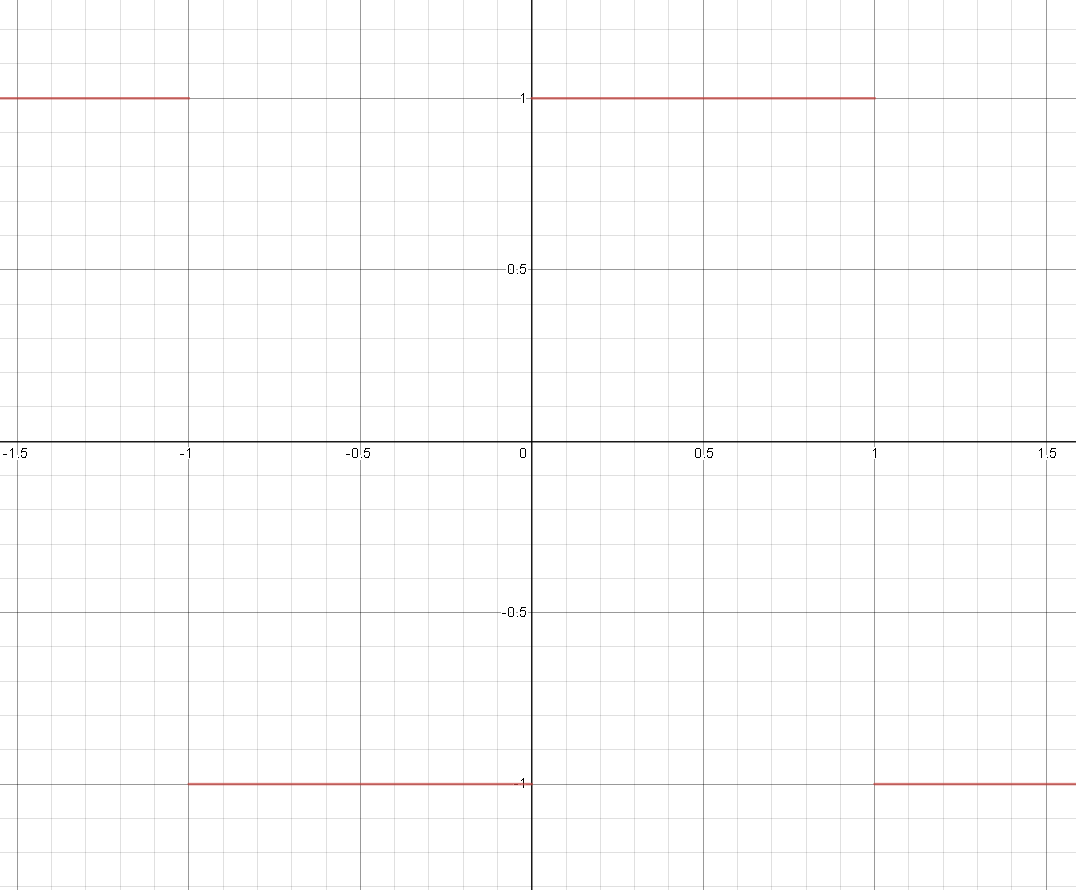
\includegraphics[scale=.175]{ExampleF} 
$$
a_n = \frac{1}{\pi} \left( \int_{0}^{\pi}\cos nt\ dt - \int_{-\pi}^{0} \cos nt\ dt\right) =0
$$
$$
b_n = \frac{1}{\pi} \left( \int_{0}^{\pi} \sin nt\ dt - \int_{-\pi}^{0} \sin nt\ dt\right) 
$$

\indk $\displaystyle \frac{1}{\pi} \left( \frac{1-\cos n\pi}{n} + \frac{1-\cos n\pi}{n}\right)= \frac{2}{\pi n}(1 - \cos n \pi)$

\indu $\displaystyle =\frac{2}{\pi n}(1-(-1)^n)= b_n$\\

\indd $\displaystyle f(t)= \frac{a_n}{2} + \sum_{n+1}^{\infty}[a_n \cos nt + b_n \sin nt] $

\indd $\displaystyle f(t)=\sum_{n+1}^{\infty} \frac{2}{\pi n}(1-(-1)^n)= b_n$

\indf $= \frac{4}{\pi} \sin t+ \frac{4}{3\pi} \sin 3t+ \frac{4}{5\pi} \sin 5t+ .....$


\newpage
\underline{How to shorten Process}:
\begin{enumerate}
\item If $f(t)$ is an even function

\indb $\rightarrow f(t)= \frac{a_n}{2} + \sum_{n+1}^{\infty}a_n \cos nt$

\indd all $b_n$ are zero

\item If $f(t)$ is an odd function

\indb $\rightarrow f(t)= \sum_{n+1}^{\infty}abn \sin nt$

\indd all $a_n$ are zero

\item If $f(t)$ is an even function

\indb $\rightarrow a_n = \frac{2}{\pi} \int_{0}^{\pi} f(t) \cdot \cos nt\ dt$


\item If $f(t)$ is an even function

\indb $\rightarrow b_n = \frac{2}{\pi} \int_{0}^{\pi} f(t) \cdot \cos nt\ dt$

\end{enumerate}

\exa Find the Fourier series

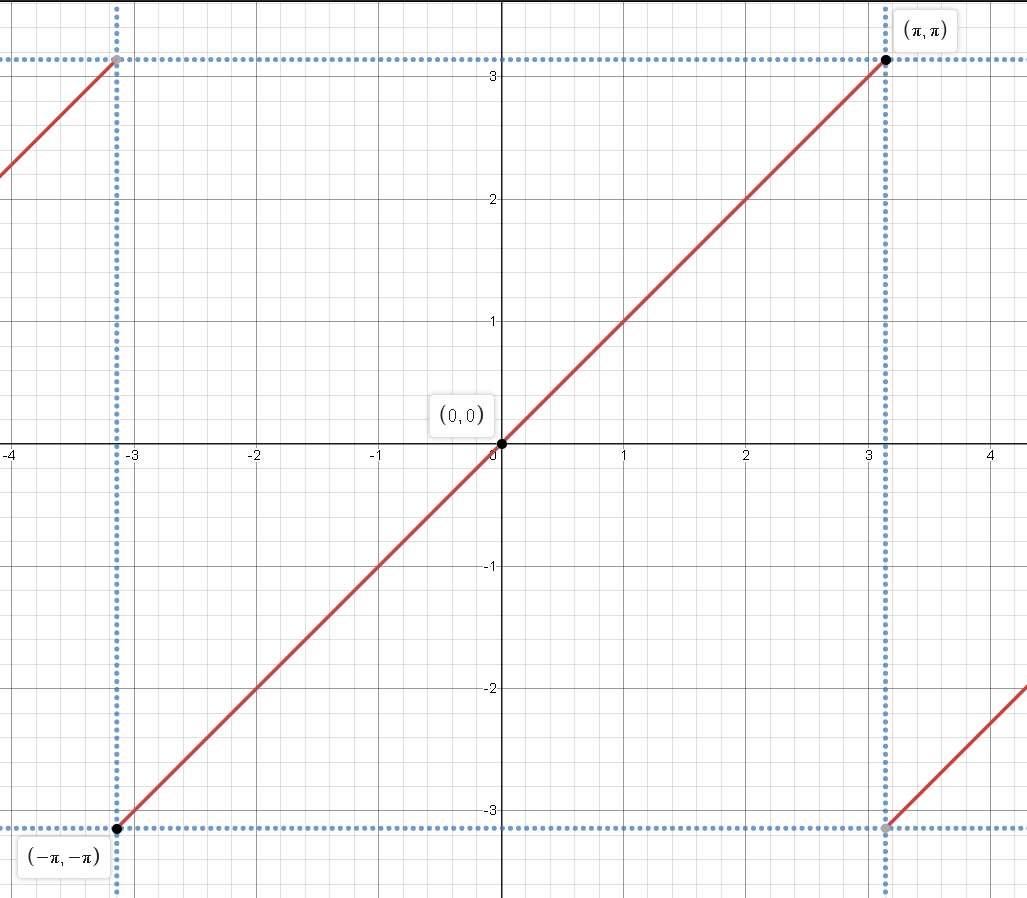
\includegraphics[scale=.25]{ExampleF1}

\indh $b_n = \frac{2}{\pi} \int_0^\pi t \sin t \ dt$

\indh $b_n = \frac{2}{\pi} \left[ -t\frac{\cos nt}{n} \vert^\pi_0 - \int_0^\pi \frac{-\cos nt}{n} \ dt \right]$

\indh $b_n = \frac{2}{\pi} \left[ \frac{-\pi}{n}(-1)^n  + \frac{\sin nt}{n^2} \vert^\pi_0 \right]$

\indh $b_n = \frac{2}{n} (-1)^{n+1}$\\

\indd $\displaystyle f(t) = \sum_{n=1}^{\infty}\frac{2}{n}(-1)^{n+1}\sin nt$

\begin{theorem}
If $f$ is continuous at $t_0$, then $f(t_0) =$ sum of F.S.

If $f$ has a jump discontinuity, then F.S.= midpoint of the jump.
\end{theorem}
\newpage

\underline{Extension 1}: period is 2L
\begin{equation}
\cos \frac{n\pi}{L}t \ \ \ \ \ \ \ a_n=\frac{1}{L} \int_{-L}^{L} f(t) \cdot \cos \frac{n \pi}{L}t\ dt
\end{equation}

\begin{equation}
\sin \frac{n\pi}{L}t \ \ \ \ \ \ \ b_n=\frac{1}{L} \int_{-L}^{L} f(t) \cdot \sin \frac{n \pi}{L}t\ dt
\end{equation}

\underline{Extension 2}: if $f$ is defined on $(0,L]$\\

\indb Periodic Extension:

\indc Either odd or even extensions making it periodic on $[-L,L]$, now do a F.S.

\subsubsection{Using Fourier Series to Solve Differential Equations}

\exa Use $\displaystyle f(t)= \frac{1}{2}+\frac{2}{\pi}\sum_{n=1}^{\infty}\frac{\sinp{(2n+1)\pi t}}{2n+1}\ $ to solve $\ x''+\omega_0x=f(t)$

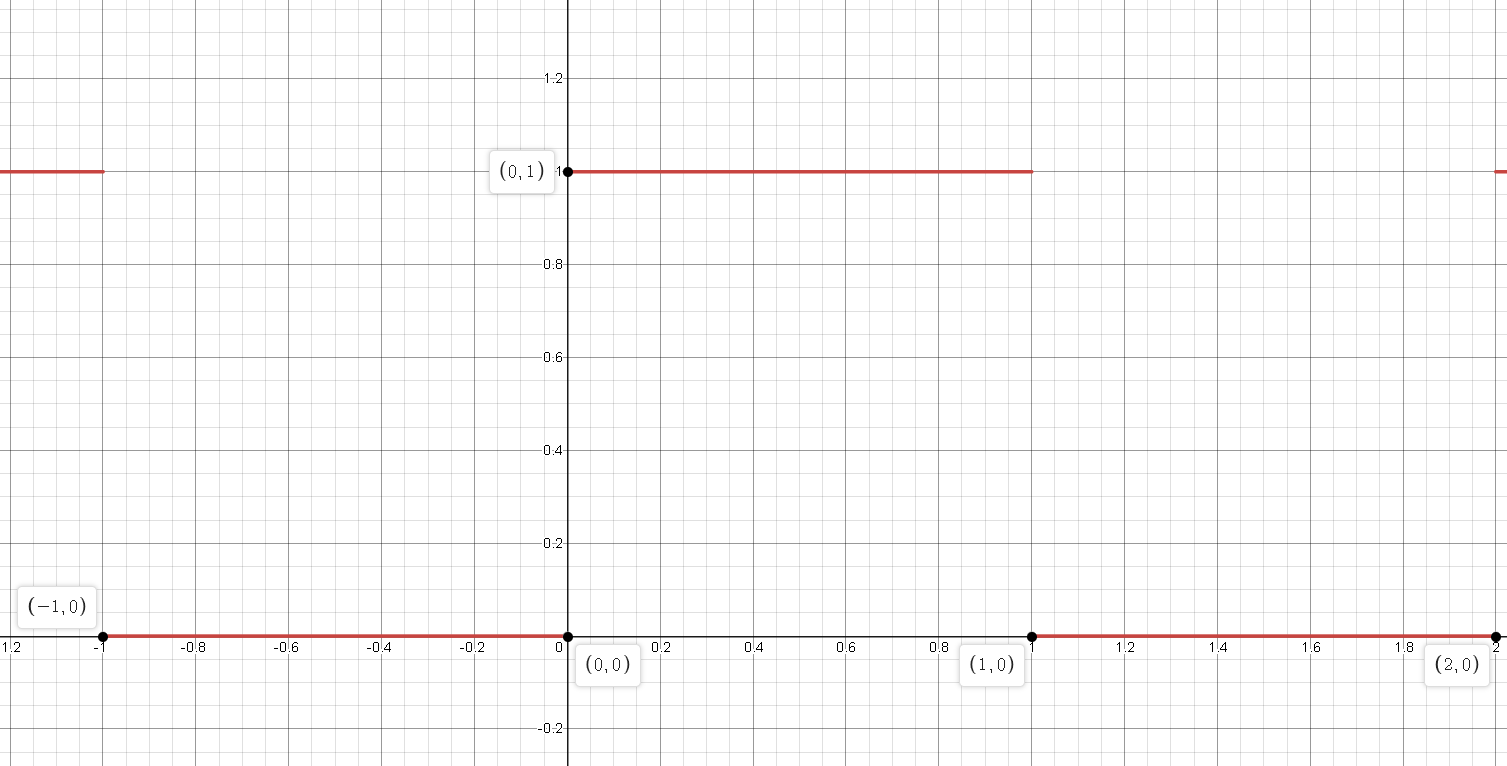
\includegraphics[scale=.25]{ExampleF2} 

\indd Knowing that if $f(t)= \sin \omega t$, then $x_p=\frac{\sin \omega t}{\omega_0^2-\omega^2}$

\indj $f(t)= \cos \omega t \ \ \ \ \ \ \ \ \ x_p=\frac{\cos \omega t}{\omega_0^2-\omega^2}$\\

\underline{More General}: If $\displaystyle f(t)= \frac{a_0}{2}+\sum_{n=1}^{\infty}a_n \cos \omega_nt + b_n \sin \omega_nt\ \ \ \ \ \ \omega_n=\frac{n \pi}{L} $ 


$$  x_p= \frac{a_0}{2 \omega_0^2}+\sum_{n=1}^{\infty} \frac{a_n \cos \omega_nt}{\omega_0^2-\omega_n^2} + \frac{b_n \sin \omega_nt}{\omega_0^2-\omega_n^2} $$

If $f$ is the sum of a bunch of functions, the particular solution will be the sum of the individual solutions because the ODE is linear. The constant term in front is treated as a cosine when $\omega_n = 0$\\

\underline{Another Method} if $\displaystyle f(t)=\frac{a_0}{2}+\sum_{n=1}^{\infty}b_n\sin nt$

Assume a solution in the form $ x_p=c_0+\sum_{1}^{\infty}c_n\sin nt$

\indk $ x_p=\ \  \ \ \ \ \sum_{1}^{\infty}-c_n n^2\sin nt$

\indd $\displaystyle c_0+\sum_{1}^{\infty}c_n[\sin nt -n^2\sin nt] =\frac{a_0}{2}+\sum_{n=1}^{\infty}b_n\sin nt$

\begin{equation}
c_0=\frac{a_0}{2}\ \ \ \ \ \ c_n=\frac{b_n}{1-n^2}
\end{equation}



\subsection{Laplace Transform}
Start with a power series
\begin{equation}
\sum_{n=0}^{\infty}a(n)x^n=A(x)
\end{equation}
The continuous analogue where $n=0,1,2,... \rightarrow 0\leq t \leq \infty$
\begin{equation}
\int_{0}^{\infty}a(t)x^t \ dt = A(x)
\end{equation}

\indu $x=e^{\ln x}$

\indu $x^t=\left(e^{\ln x}\right)^t$

\indt $0 \leq x \leq 1\ $ we want $\int$ to converge

\indu $\ln x < 0$

\indu $-s =\ln x $

\underline{Laplace Transform}:
\begin{equation}
\int_{0}^{\infty}f(t)e^{-st} \ dt = F(s)
\end{equation}
\begin{equation}
\mathscr{L}\{ f(t) \} = F(s)
\end{equation}

Linear Transform
\begin{equation}
\mathscr{L}(f+g)=\mathscr{L}(f)+\mathscr{L}(g)
\end{equation}
\begin{equation}
\mathscr{L}(c\cdot f)= c \cdot \mathscr{L}(f)
\end{equation}

\indb Because the integral is linear operator.\\

\exa $\mathscr{L}(1)$
$$ \int_0^\infty e^{-st} dt = \lim_{r \rightarrow \infty}\frac{e^{-st}}{-s} \biggr\rvert^{r}_0$$

\indm $\displaystyle = \lim_{r \rightarrow \infty}\frac{e^{-sr}}{-s} - \frac{e^0}{-s}$

\indm $= \frac{1}{s}, \ \ s > 0$

Exponential Shift Formula
\begin{equation}
e^{at}f(t)\longsquiggly F(s-a)
\end{equation}

\begin{proof}
\begin{equation}
\mathscr{L}(e^{at}f(t))=\int_0^\infty e^{at}f(t)e^{-st}\ dt
\end{equation}
\begin{equation}
\int_0^\infty e^{-(s-a)t}f(t) \ dt
\end{equation}
This is just a Laplace Transform in terms of $s-a$.
\end{proof}
$$\mathscr{L}(e^{at})=\frac{1}{s-a},\ \ s>a $$
\newpage

\exa $\mathscr{L}(\sin at\ $ and $\cos at )$\\

\indd $\cos at = \frac{e^{iat}+e^{-iat}}{2}$

\indd $\mathscr{L}(\cos at) =\frac{1}{2} \mathscr{L}(e^{iat})+\frac{1}{2}\mathscr{L}(e^{-iat})$

\indh $= \frac{1}{2}\left( \frac{1}{s-ia} + \frac{1}{s+ia}\right) $\\

\indd $\displaystyle \mathscr{L}(\cos at) =\frac{s}{s^2+a^2}$

\indd $\displaystyle \mathscr{L}(sin at) =\frac{a}{s^2+a^2} $\\

\exa Find $\mathscr{L}^{-1}$ of $\frac{1}{s(s-3)}$\\

By partial fraction decomp.

\indd $\displaystyle \frac{1}{s(s-3)} = \frac{\frac{1}{3}}{s}+ \frac{\frac{-1}{3}}{s+3}$

\indf $\leadsto \mathscr{L}^{-1} \leadsto \ \frac{1}{3}-\frac{1}{3}e^{-3t}$\\


\exa $\mathscr{L}(t^n)$\\

$$ \int_0^\infty t^ne^{-st} dt = t^n \frac{e^{-st}}{-s} \biggr\rvert^{\infty}_0 -\int_0^\infty nt^{n-1} \frac{e^{-st}}{-s} dt $$

$$ = 0 +\frac{n}{s} \int_0^\infty t^{n-1} e^{-st} dt  $$

$$ = \frac{n}{s} \mathscr{L}(t^{n-1}) $$

\indd $ \mathscr{L}(t^{n})= \frac{n}{s} \mathscr{L}(t^{n-1})= ... = \frac{n!}{s^n} \mathscr{L}(t^{0})$

$$ \mathscr{L}(t^{n}) = \frac{n!}{s^{n+1}}$$

\subsubsection{Using Laplace Transforms to Solve Linear ODEs}

We need a condition that guarantees that $\mathscr{L}$

Growth Condition:
\begin{equation}
\absp{f(t)} \leqslant Ce^{kt}\ \ \ C, k > 0
\end{equation} 
\indn Must be true all $t>0$

\indj $f(t)$ must be of exponential type

\exa $t^n$

\indd $\displaystyle \lim_{t \rightarrow \infty} \frac{t^n}{e^{kt}} = 0$

\indd $\mathscr{L}$ does exist
\newpage

\exa $\frac{1}{t}$

$$ \int_0^\infty \frac{e^{-st}}{t} dt$$

\indj Doesn't converge at $t=0$

\indj $\frac{1}{t}$ is not of exponential type\\

\indj $e^{t^2}$ is also not of exponetial type\\

\underline{Solving ODEs}: \inda [$\mathscr{L}(y(t))=\mathit{Y}(s)$]
\begin{equation}
y''+Ay'+By=h(t)
\end{equation}

\indo $\downarrow \mathscr{L}$

\begin{equation}
\mathit{Y}=\frac{p(s)}{q(s)}
\end{equation}

\indo $\downarrow \mathscr{L}^{-1}$

\begin{equation}
y(t)=y
\end{equation}

\indc Laplace Transform of a Derivative

\begin{equation}
\mathscr{L}(f'(t))
\end{equation}
\begin{equation}
=\int_0^\infty f'(t)e^{-st} dt
\end{equation}

\begin{equation}
=f(t)e^{-st} \biggr\rvert^{\infty}_0 +s \int_0^\infty f(t)e^{-st} dt
\end{equation}

\begin{equation}
=\lim_{t \rightarrow \infty} \frac{f(t)}{e^{st} } - \frac{f(0)}{1} + sF(s)
\end{equation}\\

\begin{equation}
\mathscr{L}(f'(t))=sF(s) -f(0)
\end{equation}
\begin{equation}
\mathscr{L}(f''(t))=s^2F(s) -sf(0)-f'(0)
\end{equation}\\

\exa $y''-y=e^{-y},\ \ \ \ y(0)=1\ y'(0)=0$\\

\indd $\lap (y''-y)= \lap (e^{-t})$

\indd $s^2Y-s \cdot 1 - 0 - Y = \frac{1}{s+1}$ Plugged in initial conditions.

\indd $Y \cdot (s^2-1) = \frac{1}{s+1}+s $

\indd $Y \cdot (s^2-1) = \frac{s^2+s+1}{s+1}$

\indd $Y   = \frac{s^2+s+1}{(s+1)^2(s-1)}$

\indd $Y   = \frac{-.5}{(s+1)^2}+ \frac{.25}{s+1}+\frac{.75}{s-1}$


\indd $y(t) = \lap^{-1}\left(\frac{-.5}{(s+1)^2}+ \frac{.25}{s+1}+\frac{.75}{s-1}\right)$\\

\inda $ y= \frac{1}{4}e^{-t}+\frac{3}{4}e^t-\frac{1}{2} te^{-t} $

\subsubsection{Laplace Transforms for ODEs with Jump Discontinuities}
\indb $u(t)$ is the unit step function \indf  $u(t-a)=u_a(t)$

\includegraphics[scale=.25]{unit} \inda \includegraphics[scale=.25]{unita}\\



$u_{ba}(t)$ is the unit box function $=u_b(t)-u_a(t)$

\includegraphics[scale=.25]{unitb}


\begin{equation}
\lap (u(t)) = \int_0^\infty e^{-st} u(t) \ dt = \frac{1}{s},\ \ s>0
\end{equation}
\begin{equation}
\lap(1) = \frac{1}{s} = \lap (u(t))
\end{equation}

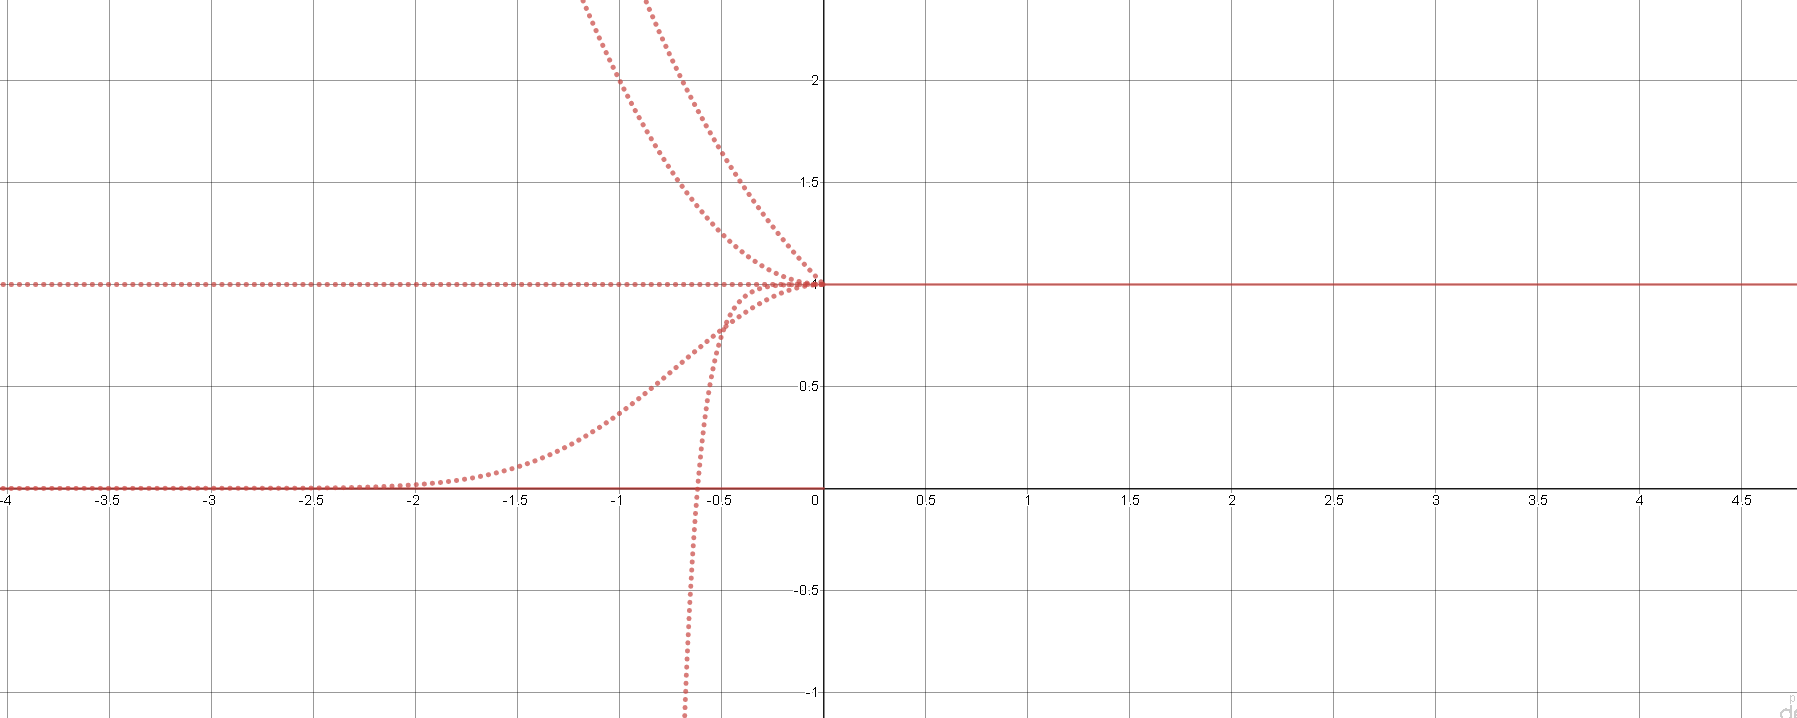
\includegraphics[scale=.25]{tails}

All these functions have the same $\lap$,  $\lap$ doesn't care about $x<0$.

\newpage

Now if $\lap(f(t))=F(s)$

\begin{equation}
\lap^{-1}(F(s))= u(t)\cdot f(t)
\end{equation}

Formula for $\lap (f(t-a))$ in terms of $f(t)$ doesn't exist

\indd 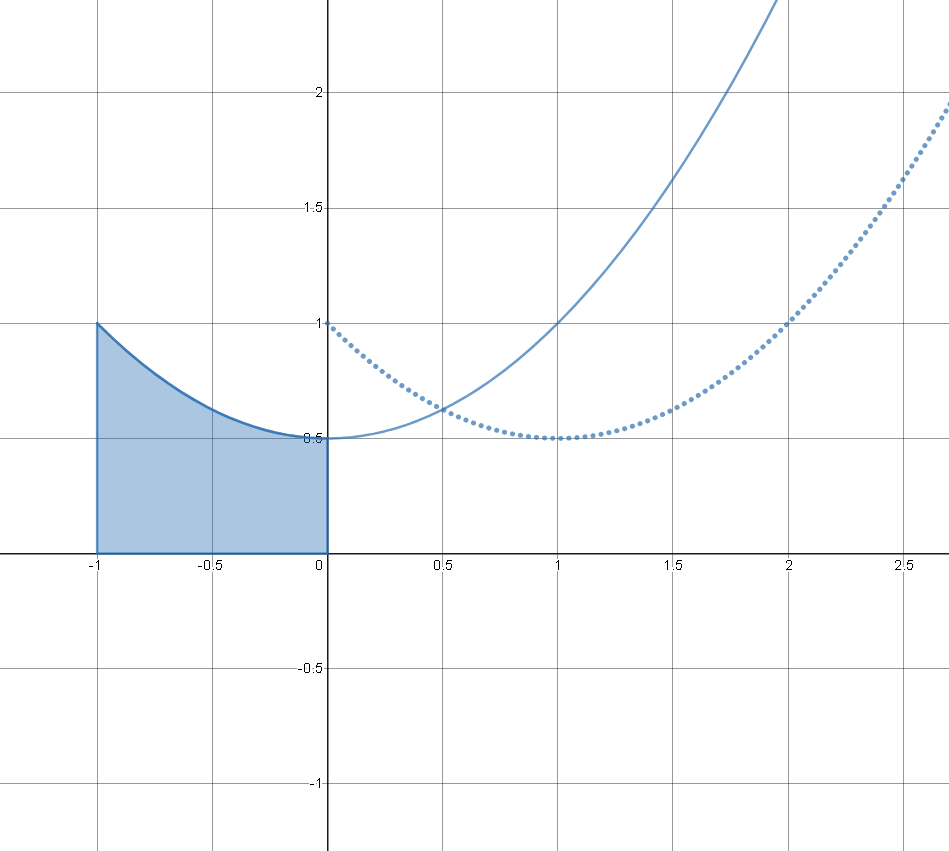
\includegraphics[scale=.25]{tran}

\indd The shaded blue piece is not used for $f(t)$

\indd however it will be needed for $f(t-a)$\\

We can find a formulas for $u(t-a)\cdot f(t-a)$
\begin{equation}
\lap(u(t-a)\cdot f(t-a))=e^{-as}F(s)
\end{equation}
\begin{equation}
\lap(u(t-a)\cdot f(t))=e^{-as}\lap(f(t+a))
\end{equation}
 \begin{proof}
 \begin{equation}
 \int_0^\infty e^{-st}u(t-a)f(t-a) dt\ \ \ \ \ \ \ t_1=t-a
 \end{equation}
 \begin{equation}
 \int_{-a}^\infty e^{-s(t_1+a)}u(t_1)f(t_1) dt_1 = e^{-as} \int_a^\infty e^{-st_1}u(t_1)f(t_1) dt_1
 \end{equation}
 \indq $u(t)$ is zero when negative,bound simplified
 
 \begin{equation}
 e^{-as} \int_a^\infty e^{-st_1}f(t_1) dt_1
 \end{equation}
 \begin{equation}
 e^{-as}F(s)
 \end{equation}
 
 \begin{equation}
 u(t-a)\cdot f(t-a) \leadsto e^{-as}\lap(f(t))\ \ \ \ \begin{small}\textrm{ replace t by t+a in f}
 \end{small}
 \end{equation}
 \begin{equation}
 u(t-a)\cdot f(t) \leadsto e^{-as}\lap(f(t+a))
 \end{equation}
 \end{proof}
 
 \exa $\lap (u_{ab}(t))$\\
 
 \indd $\lap(u(t-a))-\lap(u(t-b))$
 
  \indc $\displaystyle \frac{e^{-as}}{s}-\frac{e^{-bs}}{s}$

 \newpage
 
 \exa $\lap u(t-1) \cdot t^2$\\
 
 \indd $=e^{-s}\lap (t+1)^2$
 
 \indd $=e^{-s}\lap (t^2+2t+1)$

 \indd $=e^{-s} (\frac{2}{s^2}+\frac{2}{s^2}+\frac{1}{s})$\\

 \exa $\displaystyle \lap^{-1}\left(\frac{1+e^{-\pi s}}{s^2+1}\right)$\\
 
\indd $\lap^{-1} \frac{1}{s^2+1}+ \frac{e^{-\pi s}}{s^2+1}$
 
\indd $u(t)\sin t + u(t-\pi)\sinp{t-\pi}$ 
 
\indd $u(t)$ because we need a unique solution of this in order for formulas to work\\
 
\indb $f(t)=\sin t \ \ \ 0\leq t \leq \pi$
 
 \indb $\  \ \ \ \ \ \ \ 0 \ \ \ \ \  \ \ \ \ \ \ t > \pi$

 \newpage
\subsection{Convolution}
 
 \inda Convolution 
 \begin{equation}
 f(t) * g(t)
 \end{equation}
 
 Given
 
 $\displaystyle F(s) = \int_0^\infty e^{-st} f(t)dt$
 
 $\displaystyle G(s) = \int_0^\infty e^{-st} g(t)dt$
 
 
 \begin{equation}
 F(s)G(s)=\int_0^\infty e^{-st}(f*g)dt
 \end{equation}
 
 Why should a formula for $f*g$ exist
 
 $\displaystyle F(x) = \sum_0^\infty a_n x^n$
 
 $\displaystyle G(x) = \sum_0^\infty b_n x^n$
\begin{equation}
F(x)G(x)=\sum_0^\infty c_n x^n
\end{equation}

\indd $(a_0 + a_1x + a_2x^2 ...)(b_0 + b_1x + b_2x^2 ...)$

\indf $x^0 \indc x^1 \inde x^2 ...$

\inde $\ \ a_0b_0\ \ \ (a_0b_1+b_1a_0)\ \ (a_0b_2+a_1b_1+a_2b_0)...$

\begin{equation}
c_n=\sum_{t=0}^n a_tb_{n-t}
\end{equation}

Back to $\lap$

\begin{equation}
f*g = \int_0^t f(u)g(t-u)\ du
\end{equation}
\indu Remember $f*g=g*f$\\

\exa $t^2*t$ \indm $t^2*t$

\indt $\vee \lap$

\indd $\int_0^t u^2(t-u)\ du$ \indj $\frac{2}{s^3}\cdot \frac{1}{s^2} = \frac{2}{s^5}$\\

\indd $\frac{t^4}{3} - \frac{t^4}{4} = \frac{t^4}{12}$

\inds $\lap^{-1}(\frac{2}{s^5})=\frac{t^4}{12}$\\


\exa $f(t)*1$\\

\indd $=\int_0^t f(u)1 du$\\

\indd $=\int_0^t f(u)\ du$

\newpage

\begin{proof}\begin{equation}
F(s)G(s)= \int_0^\infty e^{-st} (f*g)\ dt
\end{equation}
\begin{equation}
F(s)G(s)= \int_0^\infty e^{-su} f(u) \ dt \cdot \int_0^\infty e^{-sv} g(v)\ dt
\end{equation}
\begin{equation}
=\int_0^\infty \int_0^\infty  e^{-s(u+v)}f(u)g(v)\ du\ dv
\end{equation}

\indu $t=u+v$

\indu $u=u\ \ \ \ \ v=t-u$
\begin{equation}
\int_0^\infty \int_0^t e^{-st} f(u) g(t-u) \ du\ dt
\end{equation}

\inds $J= \begin{vmatrix}
1 & 0 \\
-1 & 1 
\end{vmatrix}  =1$
\begin{equation}
=\int_0^\infty e^{-st} \int_0^t f(u)g(t-u) \ du \ dt
\end{equation}
\begin{center}
The middle is the formula for convolution.
\end{center}
\end{proof}

\exa Radioactive waste is dumped. $f(t)$ is the dump rate where $t=$ years\\



Starting at $t=0$

Remembering radioactive decay, at time $t$, how much waste is in the dump?\\

$A_0 e^{-kt}$ is the amount left at time $t$

\indm Amount dumped on $[u_i, u_{i+1}]$

\indn $\approx f(u_i)\cdot \Delta u$

By time $t$, it has decayed to: $f(u_i) \Delta u \cdot e^{-k(t-u_i)}$

\indb Total

$$= \lim_{\Delta u \rightarrow 0} \sum_{i=1}^{n} f(u_i)e^{-k(t-u_i)} \Delta u  $$

$$= \int_0^t f(u)e^{-k(t-u)} du  = f(t)*e^{-kt}$$

What if it didn't decay\\

$f(t)*1 \indb =\int_0^t f(u) \ du \inda $ which is intuitive\\

$f(t)\indb * \indb g(t) \inda =$ amount of $x$ at time $t$\\

prod. of $x \ \ \ \ $ how $x$ changes

\newpage
\subsection{Dirac-Delta Function}

\inda Force = force $\times $ time $[a,b]$

Constant force

\indc Impulse $= F \cdot (b-a)$

\includegraphics[scale=.25 ]{spring} y

Lets say required constants are 1 and a unit impulse is applied.

This is modeled by 
\begin{equation}
y''+y=\frac{1}{h}u_{0h}(t)
\end{equation}

\begin{equation}
\lap\left( \frac{1}{h}u_{0h}(t)\right)
\end{equation}

\begin{equation}
\frac{1}{h} \lap\left( u(t)-u(t-h) \right)
\end{equation}

\begin{equation}
\frac{1}{h} \left( \frac{1}{s}-\frac{e^{-hs}}{s} \right)
\end{equation}

What if $h \rightarrow 0$

\begin{equation}
\lim_{h \rightarrow 0} \frac{1-e^{-hs}}{hs}
\end{equation}

\begin{equation}
\lim_{u \rightarrow 0} \frac{1-e^{-u}}{u} = \lim_{u \rightarrow 0} \frac{e^{-u}}{1} =1
\end{equation}

This is the Dirac Delta Function
\begin{equation}
\delta(t)
\end{equation}

\begin{equation}
\lap[\delta(t)]=1
\end{equation}
\begin{equation}
\int_{-\infty}^{\infty} \delta(t)\ dt =1
\end{equation}
$$ \lap[u(t)f(t) * \delta (t)] = F(s) \cdot 1$$

$$ \lap[u(t)f(t) ] = F(s) $$

\begin{equation}
u(t)f(t) * \delta (t) = u(t)f(t)
\end{equation}

$\delta (t)$ is the identity element of convolution

\newpage
\exa $y''+y=A\delta (t-\frac{\pi}{2})\inda   y(0)=1,\ \ y'(0)=0$

``kicked with impulse A at time $\frac{\pi}{2}$''\\

\indd $s^2Y-s+Y=Ae^{-\frac{\pi}{2}s}$

\indd $Y=\frac{s}{s^2+1} \frac{Ae^{-\frac{\pi}{2}s}}{s^2+1}$

\indd $y=\cos t + u(t-\frac{\pi}{2})A\sinp{t-\frac{\pi}{2}}$\\

$y=\cos t \indc 0 \leq t \leq \frac{\pi}{2}$

$\inda (1-A)\cos t\ \ \ \ \ \ t \geq \frac{\pi}{2} $\\

\begin{equation}
y''+ay'+by=f(t) \inda   y(0)=0,\ \ y'(0)=0
\end{equation}
\begin{equation}
s^2Y+asY+bY=F(s)
\end{equation}
\begin{equation}
Y=F(s) \cdot \frac{1}{s^2+as+b}
\end{equation}
\indt $\frac{1}{s^2+as+b} = W(s)$ Transfer function
\begin{equation}
y(t)=f(t) * \lap^{-1}\left(\frac{1}{s^2+as+b}\right)
\end{equation}
\indt $\lap^{-1}\left(\frac{1}{s^2+as+b}\right) = w(t)$ Weight function

\begin{equation}
y(t)=\int_0^t f(u) \cdot w(t-u)\ du
\end{equation}

But what is $w(t)$, well imagine the input being the Dirac Delta Function
\begin{equation}
y''+ay'+by=\delta(t) \inda   y(0)=0,\ \ y'(0)=0
\end{equation}
\begin{equation}
s^2Y+asY+bY=1
\end{equation}
\begin{equation}
Y=\frac{1}{s^2+as+b}
\end{equation}
\begin{equation}
y(t)=w(t)
\end{equation}
\newpage

\section{Systems of Ordinary Differentials Equations}
\subsection{First Order Systems of ODEs}
\begin{equation}
x'=f(x,y,t)=\dert{x}
\end{equation}
\begin{equation}
y'=g(x,y,t)=\dert{y}
\end{equation}

$x$ and $y$ are independent variables on $t$.\\

\underline{Linear Systems}:
\begin{equation}
x'=ax+by+r_1(t)
\end{equation}
\begin{equation}
y'=cx+dy+r_2(t)
\end{equation}
\begin{equation}
x(t_0)=x_0 \inda y(t_0)=y_0
\end{equation}
 
$a,\ b,\ c,\ d\ $ can be functions of $t$. If $a,\ b,\ c,\ d\ $ are constants, the system is called a constant-coefficient system.\\

\begin{definition}
A system is Homogeneous if it has no $r_1(t)$ or $r_2(t)$.
\end{definition}

A system has as many initial conditions as the total order in the system. \\


\exa An egg in water with yolk and white stuff.

\indd $T_e(t)=$ temp. of water (constant for simplicity)

\indd $T_2(t)=$ temp. of white stuff 

\indd $T_1(t)=$ temp. of yolk\\

\indj $\displaystyle \dert{T_1}=a(T_2-T_1)  $

\indh $\displaystyle \dert{T_2}=a(T_1-T_2) + b(T_e-T_2) $\\

\indj $T_1'=-aT_1+aT_2  $

\indj $ T_2'=aT_1-(a+b)T_2+bT_e$

Lets say $T_e=0$

also a=2, b=3

\indj $T_1'=-2T_1+2T_2  $

\indj $ T_2'=\ 2T_1-5T_2$

\indj To eliminate $T_2$ \inde $\displaystyle T_2=\frac{T_1'+2T_1}{2}$\\

\indi $\displaystyle \left( \frac{T_1'+2T_1}{2} \right)'=2T_1-5\left( \frac{T_1'+2T_1}{2} \right)$

\indj $T_1''+7T_1'+6T=0$


\indf $T_1 = c_1e^{-6t}+c_2e^{-t}$

\indf $T_2 = \frac{1}{2}c_2e^{-t}-2c_1e^{-6t}$\\

\indd $T_1(0)=40$

\indd $T_2(0)=45$\\

\indd $40=c_1+c_2$

\indd $45=\frac{1}{2}c_2-2c_1$

\indc \line(1,0){100}

\indd $c_1=-10 \indb c_2=50$

$$T_1 = 50e^{-t}-10e^{-6t} $$
$$T_2 = 25e^{-t}+20e^{-6t} $$

\begin{definition} An autonomous system has no ``t''s.
\end{definition}

\indc $x'=f(x,y)$

\indc $y'=g(x,y)$\\

The solution is a parametric equations of the form

$x=x(t)$

$y=y(t)$\\

$x'$ and $y'$ give a vector field  of the velocities of the solutions.


\subsubsection{Eigenvalue Method of Solving First Order Systems of ODEs }

A different method to the first example.\\

\indm Ans. \indg Sol.

$x=T_1$ \indi $x'=-2x+2y$ \indd $x=c_1e^{-t}+c_2e^{-6t}$

$y=T_2$ \indi $y'=2x-5y$  \indd $y=\frac{c_1}{2}e^{-t}-2c_2e^{-6t}$\\

\indf Que.  \indk Sol.

\indd $\begin{pmatrix}
x \\
y
\end{pmatrix}'=\begin{pmatrix}
-2 & 2 \\
2 & -5
\end{pmatrix} \begin{pmatrix}
x \\
y
\end{pmatrix}$ \indd $\begin{pmatrix}
x \\
y
\end{pmatrix}=c_1\begin{pmatrix}
1 \\
\frac{1}{2}
\end{pmatrix}e^{-t}+c_2\begin{pmatrix}
1 \\
-2
\end{pmatrix}e^{-6t}$\\

Process:\\

\indd Substitute 

$$ \begin{pmatrix}
x \\
y
\end{pmatrix}=\begin{pmatrix}
a_1 \\
a_2
\end{pmatrix}e^{\lambda t} $$

$$ \lambda \begin{pmatrix}
a_1 \\
a_2
\end{pmatrix}e^{\lambda t}= \begin{pmatrix}
-2 & 2 \\
2 & -5
\end{pmatrix} \begin{pmatrix}
a_1 \\
a_2
\end{pmatrix}e^{\lambda t}$$

$$ \lambda \begin{pmatrix}
a_1 \\
a_2
\end{pmatrix}= \begin{pmatrix}
-2 & 2 \\
2 & -5
\end{pmatrix} \begin{pmatrix}
a_1 \\
a_2
\end{pmatrix}$$

This is now a system of equations:\\

\indd $\lambda a_1 = -2a_1+2a_2$

\indd $\lambda a_2 = 2a_1-5a_2$\\

This is 3 unkowns in 2 equations so lets treat $\lambda$ as a parameter\\

\indd $ (-2-\lambda)a_1+2a_2=0$

\indd $ 2a_1+(-5-\lambda) a_2 =0$\\

There exists a non-trivial solution if and only if:

$$ \begin{vmatrix}
-2-\lambda & 2 \\
2 & -5-\lambda
\end{vmatrix} =0$$

This is the condition $\lambda$ must satisfy\\

\indd $(\lambda +2)(\lambda +5 )-4=0$

\indd $\lambda^2 +7\lambda +6=0$

\indd $\lambda=-1, \ -6$

Notice how the quadratic equation is the same as the characteristic equation gotten from the first method. These values of $\lambda$ are called the eigenvalues of the coefficient matrix.\\

\indd $\lambda=-1$ \inda Find $a_1$ and $a_2$ \indg $\lambda=-6$\\

\indc $-a_1+2a_2=0$ \indk $4a_1+2a_2=0$

\indc $2a_1-4a_2=0$ \indk $2a_1+a_2=0$\\

Notice how one equation is a constant multiple of the other, this is an easy way to check if everything is going correctly. As these are the same equations, find any solution that works. Usually substitute 1 in and see what value the other unknown is. Then put the two values into what is known as a eigen vector. Then multiply by e to the eigenvalue times t.\\

\indc $a_2=1 \ \rightarrow \ a_1=2$ \indi $a_2=-2\ \rightarrow \ a_1=1$

\inde $\begin{pmatrix}
2 \\
1
\end{pmatrix}e^{-t}$ \indl $\begin{pmatrix}
1 \\
-2
\end{pmatrix}e^{-6t}$\\

By superposition:

$$\begin{pmatrix}
x \\
y
\end{pmatrix}=c_1\begin{pmatrix}
1 \\
\frac{1}{2}
\end{pmatrix}e^{-t}+c_2\begin{pmatrix}
1 \\
-2
\end{pmatrix}e^{-6t} $$

If a different eigen vector was chosen, it would have to be a constant multiple of the previous, which can be factored out into the unknown constants in front.  

\newpage
\noindent \underline{In General}:
\begin{equation}
\begin{pmatrix}
x \\
y
\end{pmatrix}'=\begin{pmatrix}
a & b \\
c & d
\end{pmatrix} \begin{pmatrix}
x \\
y
\end{pmatrix}
\end{equation}
\inda Trial
\begin{equation}
\begin{pmatrix}
a_1 \\
a_2
\end{pmatrix}e^{\lambda t} 
\end{equation}\\
\begin{equation}
\lambda \begin{pmatrix}
a_1 \\
a_2
\end{pmatrix}= A \begin{pmatrix}
a_1 \\
a_2
\end{pmatrix}
\end{equation}
\inda Solvable if:
\begin{equation}
\begin{vmatrix}
a-\lambda & b \\
c & d-\lambda
\end{vmatrix} =0
\end{equation}
\begin{equation}
\lambda^2-(a+b)\lambda +ad-bc=0
\end{equation}
\inda This the characteristic equation which can also be written as:
\begin{equation}
\lambda^2+ \lambda \trace A  +\det A =0
\end{equation}
\inda Where det is the determinant and trace is the sum of the main diagonal.\\

The two roots $\lambda_1 $ and $\lambda_2 $ (for now assume real and distinct) are the eigenvalues for A.\\

For each $\lambda_i$, find the associated:
\begin{equation}
\vec{\alpha}_i=\begin{pmatrix}
a_{1i} \\
a_{2i}
\end{pmatrix}
\end{equation}
\inda By solving the system:
\begin{equation}
\begin{pmatrix}
a-\lambda & b \\
c & d-\lambda
\end{pmatrix} \cdot \begin{pmatrix}
a_1 \\
a_2
\end{pmatrix} =0
\end{equation}
The general solution is now in the form:
\begin{equation}
\begin{pmatrix}
x \\
y
\end{pmatrix}=c_1\begin{pmatrix}
a_{11} \\
a_{21}
\end{pmatrix}e^{\lambda_1 t}+c_2\begin{pmatrix}
a_{12} \\
a_{22}
\end{pmatrix}e^{\lambda_2 t} 
\end{equation}
\newpage

\noindent {More in general}:
\begin{equation}
\begin{pmatrix}
x \\
y \\
\vdots
\end{pmatrix}=\vec{x} \indf \vec{x}'=A\vec{x}
\end{equation}
\begin{equation}
\begin{pmatrix}
a & b & \dots \\
c & d & \dots \\
\vdots & \vdots & \ddots
\end{pmatrix}=A \indf \textrm{Trial}: \ \  \vec{x}=\vec{\alpha}e^{\lambda t}
\end{equation}
\begin{equation}
\begin{pmatrix}
a_1 \\
a_2 \\
\vdots
\end{pmatrix}=\vec{\alpha} \indf \lambda\vec{\alpha}=A\vec{\alpha}
\end{equation}
\begin{equation}
\begin{pmatrix}
1 & 0 & 0 & \dots \\
0 & 1 & 0 & \dots \\
0 & 0 & 1 & \dots \\
\vdots & \vdots & \vdots & \ddots
\end{pmatrix}=I \indf (A-\lambda \cdot I)\vec{\alpha}=0
\end{equation}
\begin{equation}
\indm \textrm{Chara. Eq.} \ \ \absp{A-\lambda I}=0
\end{equation}
\begin{center}
now continue with the eigenvalues as before
\end{center}

\exa Image a tank divide into 3 sections where 

\indd $X_i$ gives the temperature in tank $i$. 

\indd Any constants are 1.

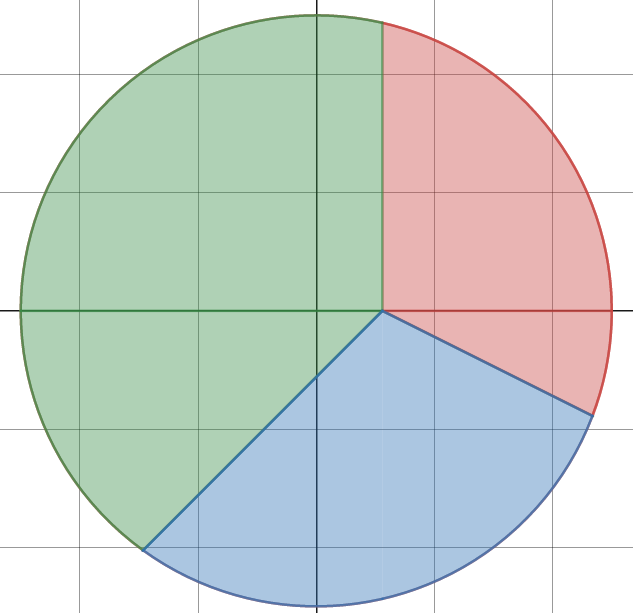
\includegraphics[scale=.25]{SODE1} \indc $ \ x_1'=a(x_3-x_1)+a(x_2-x_1)$

\indl $x_1'=-2ax_1+ax_2+ax_3$\\

\indk $x_1'=-2x_1+x_2+x_3$

\indk $x_2'=x_1-2x_2+x_3$

\indk $x_3'=x_1+x_2-2x_3$\\

$$\absp{A-\lambda I}= \begin{vmatrix}
-2-\lambda & 1 & 1 \\
1 & -2-\lambda & 1 \\
1 & 1 & -2-\lambda 
\end{vmatrix} = -(\lambda +2)^3 +2-3(-2-\lambda)=0 $$

\indq $\lambda^3 +6\lambda^2+12\lambda+8-2 -6 -3\lambda=0$

\indq $\lambda^3 +6\lambda^2+9\lambda=0$

\indq $\lambda(\lambda^2 +6\lambda+9)=0$
 
\indq $\lambda(\lambda+3)^2=0$
\newpage

The eigenvalues are $0$ and a repeated $-3$\\

\indd $\lambda=0$\\

\indd $(A-\lambda I)\vec{\alpha}=0$

\indd $A\vec{\alpha}=0$\\

\indb $-2a_1+a_2+a_3=0$

\indb $a_1-2a_2+a_3=0$

\indb $a_1+a_2-2a_3=0$

$$ \begin{pmatrix}
a_1 \\
a_2 \\
a_3
\end{pmatrix}e^{0t}=\begin{pmatrix}
1 \\
1 \\
1
\end{pmatrix} $$

\indd $\lambda=-3$\\

\indb $a_1+a_2+a_3=0$

\indb $a_1+a_2+a_3=0$

\indb $a_1+a_2+a_3=0$\\

In this case, there are two possible solutions such that one is not a constant multiple of the other:
$$ \begin{pmatrix}
1 \\
0 \\
-1 
\end{pmatrix}\ \ \textrm{or}\ \ \begin{pmatrix}
1 \\
-1 \\
0
\end{pmatrix} $$

Notice how $\begin{pmatrix}
0 \\
1 \\
-1
\end{pmatrix} $ is not a new solution. It is not a constant multiple of the other but it is a linear combination, disqualifying it. The solution now is:

$$ \begin{pmatrix}
x_1 \\
x_2 \\
x_3 
\end{pmatrix} = c_1 \begin{pmatrix}
1 \\
0 \\
-1
\end{pmatrix}e^{-3t} + c_2 \begin{pmatrix}
1 \\
-1 \\
0
\end{pmatrix}e^{-3t} + c_3 \begin{pmatrix}
1 \\
1 \\
1
\end{pmatrix} $$

\begin{definition}[Complete Eigenvalue]
If an eigenvalue $\lambda$ is repeated, but you can find enough  needed eigenvectors, then it is complete.
\end{definition}

\begin{definition}[Defective Eigenvalue]
If an eigenvalue $\lambda$ is repeated, but you can not find enough  needed eigenvectors, then it is defective.
\end{definition}

\begin{theorem}
If a real $n \times n$ matrix which is symmetric (about diagonal) then all of its eigenvalues are complete.
\end{theorem}
\newpage

\noindent \underline{Complex Eigenvalues}:

\begin{enumerate}
\item Calculate complex eigenvalues
\item Formulate solution: $\vec{\alpha}e^{(a+bi)t}$
\item Take the real and imaginary parts to get two solutions.
\end{enumerate}

\exa $ x'=x+2y$

\indd $\ \ y'=-x-y$\\

\indb $A=\begin{pmatrix}
1 & 2 \\
-1 & -1
\end{pmatrix}$\\

\indd $\lambda^2+0\lambda + (-1+2)=0$

\indd $\lambda^2+1=0$

\indd $\lambda = \pm i$\\

\indc $\lambda= i$\\

\indb $(1-i)a_1+2a_2=0$

\indb $-1a_1+(-1-i)a_2=0$

\indf $a_1=1 \rightarrow a_2=\frac{-1+i}{2}$

$$\begin{pmatrix}
1 \\
\frac{-1+i}{2}
\end{pmatrix} e^{it} = \left[ \begin{pmatrix}
1 \\
-\frac{1}{2}
\end{pmatrix}+i\begin{pmatrix}
0 \\
\frac{1}{2}
\end{pmatrix} \right] (\cos t +i \sin t)$$

Solutions:

$$\textrm{Real}\ = \begin{pmatrix}
x \\
y
\end{pmatrix}=\begin{pmatrix}
1 \\
-\frac{1}{2}
\end{pmatrix}\cos t - \begin{pmatrix}
0 \\
\frac{1}{2}
\end{pmatrix}\sin t  $$

$$\textrm{Imaginary}\ = \begin{pmatrix}
x \\
y
\end{pmatrix}=\begin{pmatrix}
0 \\
\frac{1}{2}
\end{pmatrix}\cos t + \begin{pmatrix}
1 \\
-\frac{1}{2}
\end{pmatrix}\sin t  $$

\newpage
\subsection{How to Sketch Solutions to Systems of First Order ODEs}
We will work with the cases of:
\begin{equation}
x'=-x+by
\end{equation}
\begin{equation}
y'=cx-3y
\end{equation}

\bigskip 

\underline{First Case}: $\ x'=-x+2y$

\indd $\ \  y'=-3y$\\

Solving the system yields:
$$ \begin{pmatrix}
x \\ y
\end{pmatrix}=c_1\begin{pmatrix}
1 \\ -1
\end{pmatrix}e^{-3t}+c_2\begin{pmatrix}
1 \\ 0
\end{pmatrix}e^{-t}$$

\indb 1.) There are 4 easy solutions

\indd \textcolor{purpleheart}{$c_1=\pm 1, \ \ \ c_2=0$}

\indd \textcolor{red}{$c_1=0, \ \ \ c_2=\pm 1$}


\indf These just straight lines, what about in between\\

\indb 2.)\textcolor{blue}{\begin{small}
$ \begin{pmatrix}
x \\ y
\end{pmatrix}=c_1\begin{pmatrix}
1 \\ -1
\end{pmatrix}e^{-3t}+c_2\begin{pmatrix}
1 \\ 0
\end{pmatrix}e^{-t}$
\end{small}}

\indh $\downarrow$ \indd $\searrow$ dom. as $t \rightarrow \infty$

\indh dom. as $tv \rightarrow -\infty$\\

\begin{center} 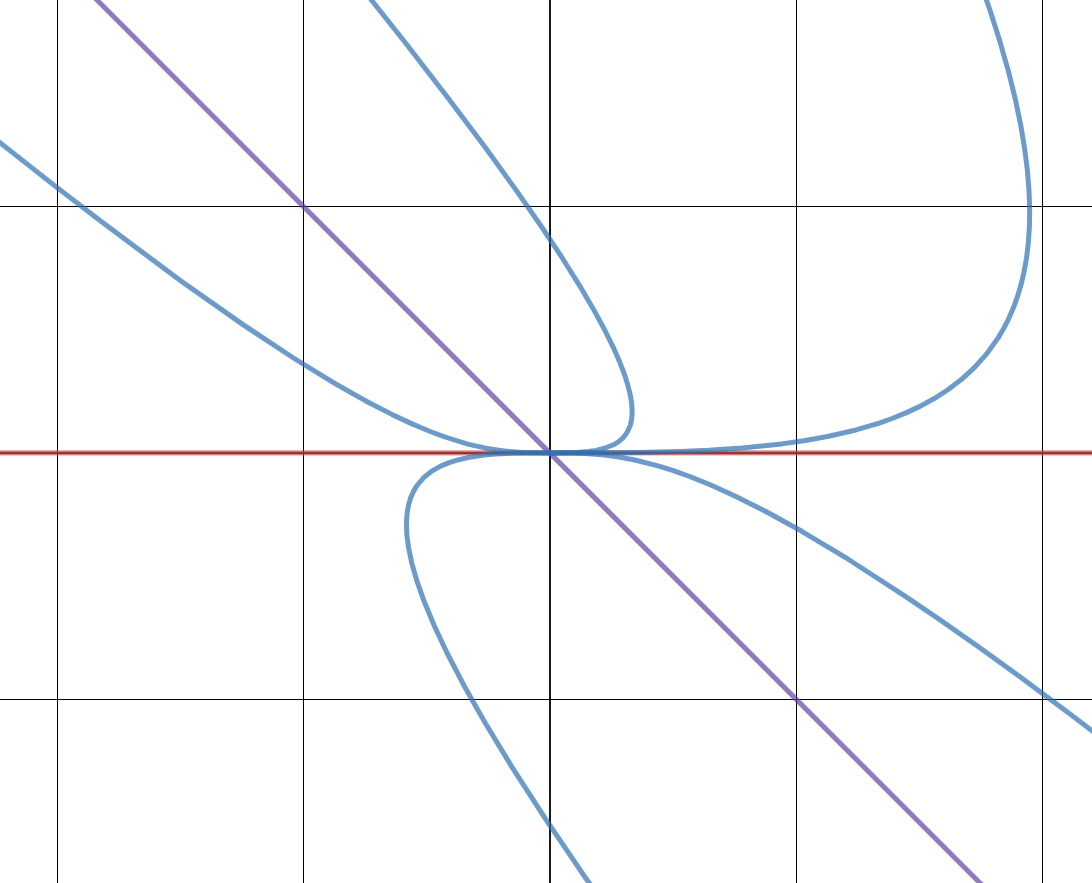
\includegraphics[scale=.25]{sketch1} \end{center}

In this case, all the lines go towards the origin as $t \rightarrow \infty$, making the origin a sync node. If the signs where flipped as in 
\begin{equation}
\begin{pmatrix}
x \\ y
\end{pmatrix}=c_1\begin{pmatrix}
1 \\ -1
\end{pmatrix}e^{\underline{3t}}+c_2\begin{pmatrix}
1 \\ 0
\end{pmatrix}e^{\underline{t}}
\end{equation}
then the curves would go all outwards from the origin, making the origin a source node.

\newpage

\exa $\ x'=-x+3y$

\indd $\ \ \ y'=5x-3y$\\

Solving the system yields:

$$ \begin{pmatrix}
x \\ y
\end{pmatrix}=c_1\begin{pmatrix}
3 \\ -5
\end{pmatrix}e^{-6t}+c_2\begin{pmatrix}
1 \\ 1
\end{pmatrix}e^{2t}$$

The four trivial solutions give line where one goes toward the origin and another away. This makes the origin a saddle point. Everything in between acts like a hyperbola.
\begin{center}
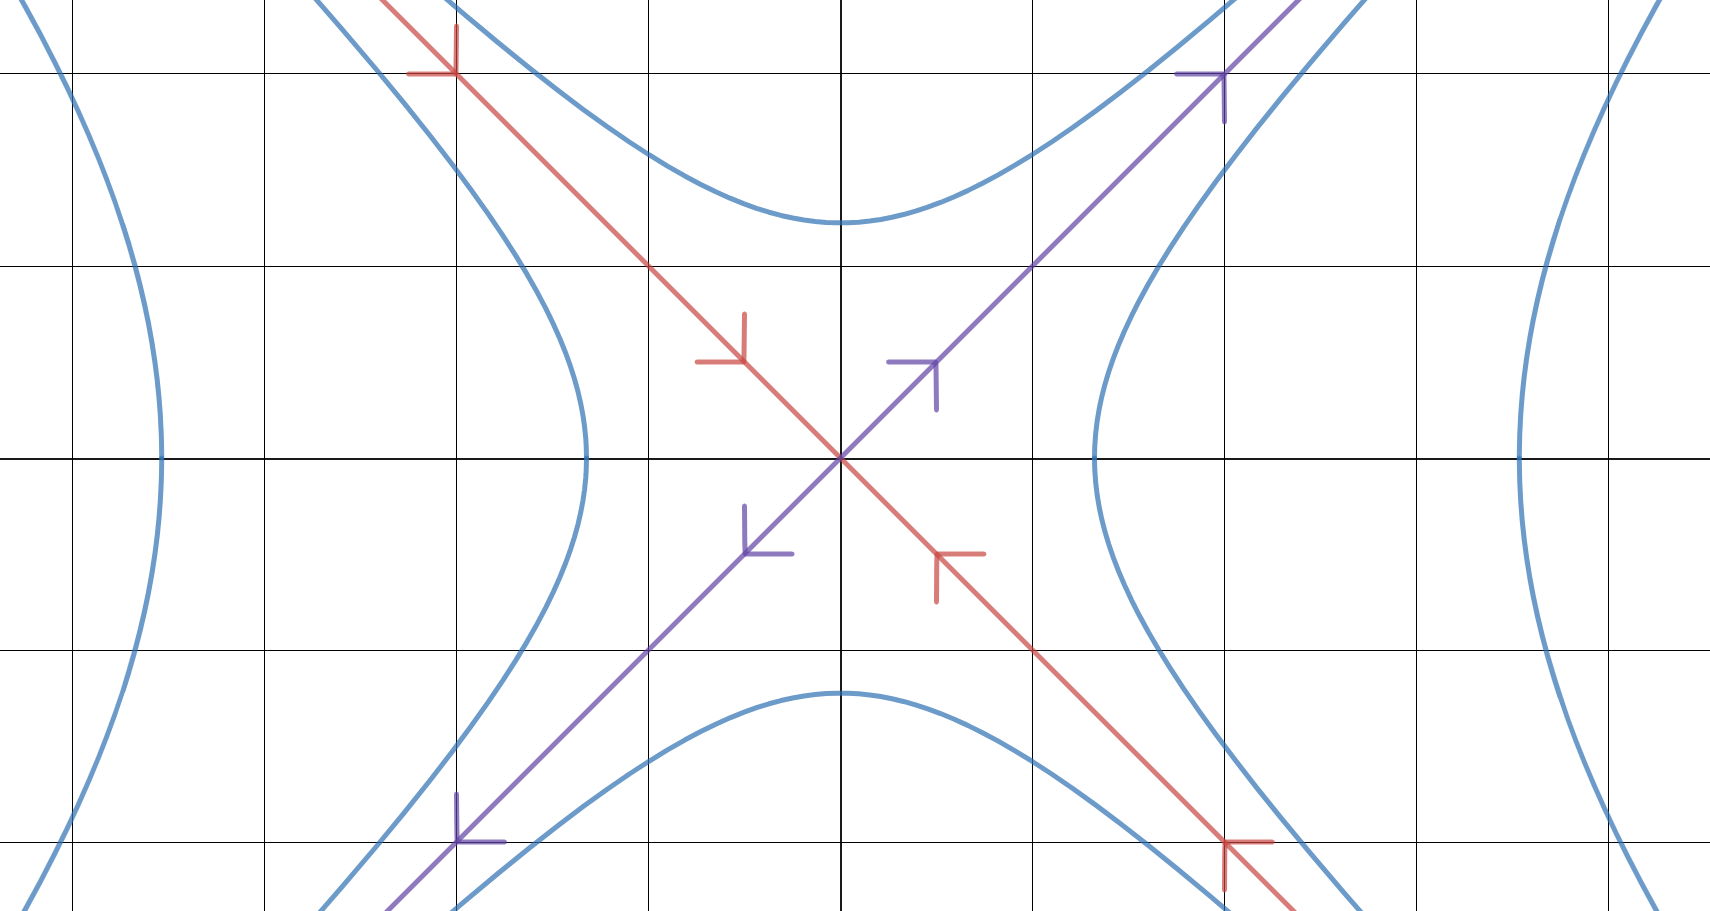
\includegraphics[scale=.25]{sketch2}\\
\end{center}

\exa Complex eigenvalues:\\

Solutions looks something like 

$$\begin{pmatrix}
x \\ y
\end{pmatrix} = c_1 \left[ \begin{pmatrix}
a_1 \\ a_2
\end{pmatrix} \cos t + \begin{pmatrix}
b_1 \\ b_2
\end{pmatrix} \sin t \right]e^{(\lambda t)}+c_2[\textrm{something similar}] $$

The $\cos t$ and $\sin t$ make circles which grow and decay because of the exponential. So essentially you get spirals. To check which direction, you plug a point into the initial problem to get a velocity vector.










\newpage
\subsection{Inhomogeneous Systems}
\inda Lets begin with the theory of Homogeneous Systems (constant coefficient matrix):
\begin{equation}
\vec{x}'=A\vec{x}
\end{equation}

\begin{theorem}
The general solution to $\vec{x}'=A\vec{x}$ is:
\begin{equation}
\vec{x}=c_1\vec{x}_1+c_2\vec{x}_2
\end{equation}
Where $\vec{x}_1$ and $\vec{x}_2$ are two solutions which linearly independent of each other and not constant multiples of each other.
\end{theorem}

\begin{theorem}
The Wronskian of two solutions
\begin{equation}
W(\vec{x}_1,\ \vec{x}_2)= \absp{\vec{x}_1\ \vec{x}_2}
\end{equation}
Either: $W(t)\equiv 0$ (if $\ \vec{x}_1, \ \vec{x}_2$ are dependent)

\inda or $W(t)$ is never 0 for any $t$.
\end{theorem}

\underline{Fundamental Matrix for the System}: $\mathbb{X}=\begin{bmatrix}
\vec{x}_1 & \vec{x}_2
\end{bmatrix}$ where $\vec{x}_1$ and $\vec{x}_2$ are two ind. solutions

\indd Properties:

\inde 1.) $\absp{\mathbb{X}}\neq 0$ for any $t$.

\inde 2.) $\mathbb{X}' = A\mathbb{X}$ 

\begin{proof}
\begin{equation}
\begin{bmatrix}
\vec{x}_1' & \vec{x}_2'
\end{bmatrix}
=A\begin{bmatrix}
\vec{x}_1 & \vec{x}_2
\end{bmatrix}=\begin{bmatrix}
A\vec{x}_1 & A\vec{x}_2
\end{bmatrix}
\end{equation}
\begin{equation}
\Leftrightarrow \vec{x}_1'=A\vec{x}_1 \ , \ \vec{x}_2'=A\vec{x}_2
\end{equation}
\end{proof}

\noindent Inhomogeneous Systems:

\indb $x'=ax+by+r_1(t)$

\indb $y'=cx+dy+r_2(t)$

\begin{equation}
\vec{x}'=A\vec{x}+\vec{r}(t)
\end{equation}


\begin{theorem}
The general solution is the sum of the solution to the homogeneous system and the particular solution.
\begin{equation}
\vec{x}_g = \vec{x}_c+ \vec{x}_p
\end{equation}
\end{theorem}
\newpage


We need a method to solve $\vec{x}'=A\vec{x}+\vec{r}$ for $\vec{x}_p$\\

\noindent \underline{Variation of Parameters}:

\begin{equation}
\vec{x}_p=v_1(t)\vec{x}_1+v_2(t)\vec{x}_2
\end{equation}
\indi Where $\vec{x}_1 $ and $\vec{x}_2$ are solutions to the homo. system.

\begin{equation}
\vec{x}_p=\mathbb{X}\vec{v}
\end{equation}

\begin{equation}
\vec{x}_p=\begin{pmatrix}
x_1 & x_2 \\
y_1 & y_2 
\end{pmatrix}\begin{pmatrix}
v_1\\
v_2
\end{pmatrix}=\begin{pmatrix}
x_1v_1 + x_2v_2 \\
y_1v_1 + y_2v_2
\end{pmatrix}
\end{equation}

Substitute into system and see what $\vec{v}$ is

\begin{equation}
\vec{x}'=A\vec{x}+\vec{r}
\end{equation}

\begin{equation}
\mathbb{X}'\vec{v} + \mathbb{X}\vec{v}' =A\mathbb{X}\vec{v}+\vec{r}
\end{equation}

\begin{equation}
A\mathbb{X}\vec{v} + \mathbb{X}\vec{v}' =A\mathbb{X}\vec{v}+\vec{r}
\end{equation}

\begin{equation}
\mathbb{X}\vec{v}' = \vec{r}
\end{equation}

\begin{equation}
\vec{v}' =\mathbb{X}^{-1} \vec{r}
\end{equation}

\begin{equation}
\vec{v} =\int \mathbb{X}^{-1} \vec{r}\ dt
\end{equation}

\begin{equation}
\vec{x}_p =\mathbb{X} \int \mathbb{X}^{-1} \vec{r}\ dt
\end{equation}\\

There isn't a Fundamental Matrix $\mathbb{X}$, any two solutions to the homo. system will work.
\begin{equation}
\vec{x}=c_1\vec{x}_1+c_2\vec{x}_2
\end{equation}
\begin{equation}
\vec{x}=\mathbb{X}\vec{c}
\end{equation}

Using that new definition of a solution, the most general FM looks like:
\begin{equation}
\begin{bmatrix}
\mathbb{X}\vec{c}_1 & \mathbb{X}\vec{c}_2
\end{bmatrix}=\mathbb{X}\begin{bmatrix}
\vec{c}_1 & \vec{c}_2
\end{bmatrix}
\end{equation}
\begin{equation}
=\mathbb{X}C
\end{equation}

\indb Where $C$ is any 2x2 constant coefficient matrix.


\newpage
\subsection{Matrix Exponentials} 

For \begin{equation}
\vec{x}'=A\vec{x}
\end{equation}

\indd We want a formula and not a algorithm.\\

For a $ 1 \times 1 $ case: $x'=ax \leadsto x=ce^{at}$

$$e^{at} = 1 + at + \frac{a^2t^2}{2!}+\frac{a^3t^3}{3!}+ .\ .\ .\ $$

$$\frac{de^{at}}{dt} = a + a^2t + \frac{a^3t^2}{2!}+\frac{a^3t^3}{3!}+ .\ .\ .\ $$

$$ \frac{de^{at}}{dt} =ae^{at}$$

So $e^{at}$ solves the $1 \times 1$ differential equation.\\

A fundamental matrix for $\vec{x}'=A \vec{x}$
\begin{equation}
\textrm{is} e^{At} : = I_n + At + \frac{A^2t^2}{2!} + \frac{A^3t^3}{3!}
\end{equation}
This is the FM because it satisfies $\mathbb{X}'=A\mathbb{X}$ and $\det \mathbb{X} \neq 0$\\

\exa $x'=y$

\indd $\ y'=x$\\

\indr $A=\begin{bmatrix}
0 & 1 \\
1 & 0
\end{bmatrix}$

\indr $A^2=\begin{bmatrix}
0 & 1 \\
1 & 0
\end{bmatrix} \cdot \begin{bmatrix}
0 & 1 \\
1 & 0
\end{bmatrix} = \begin{bmatrix}
1 & 0 \\
0 & 1
\end{bmatrix} = I_2$

\indr $A^3= I \cdot  A = A$

\indr $A^4= A^3 \cdot  A = A \cdot A = I_2$


$$e^{At} =\begin{bmatrix}
1 & 0 \\
0 & 1
\end{bmatrix} +  \begin{bmatrix}
0 & 1 \\
1 & 0
\end{bmatrix} t + \begin{bmatrix}
1 & 0 \\
0 & 1
\end{bmatrix} \frac{t^2}{2!} + \begin{bmatrix}
0 & 1 \\
1 & 0
\end{bmatrix} \frac{t^3}{3!} +\ .\ .\ .\ .\ $$


$$ \begin{bmatrix}
1 + \frac{t^2}{2!} + \frac{t^4}{4!} +... & t+\frac{t^3}{3!} + ...\\
t+\frac{t^3}{3!} + ... & 1 + \frac{t^2}{2!} + \frac{t^4}{4!}
\end{bmatrix}$$


$$ e^{At} = \begin{bmatrix}
\cosh t & \sinh t \\
\sinh t & \cosh t
\end{bmatrix} $$
\newpage

What about an initial value $\vec{x}(0)=\vec{x}_0$\\

\indd Solution
\begin{equation}
\vec{x}= e^{At} \cdot \vec{c}
\end{equation}
\begin{equation}
\vec{x}(0)= e^{A0} \cdot \vec{c}
\end{equation}
\begin{equation}
\vec{x}_0= I_2  \cdot \vec{c}
\end{equation}
\begin{equation}
\vec{x}_0= \vec{c}
\end{equation}
\begin{equation}
\vec{x}= e^{At} \cdot \vec{x}_0
\end{equation}

Matrix Exponentials don't follow standard laws of exponents:
\begin{equation}
e^{A+B} \neq e^A \cdot e^B
\end{equation}
\indd This is only true in the special case of $AB=BA$\\

Three important cases of $AB = BA$

\indb 1.) if $A=cI=\begin{bmatrix}
c & 0 \\
0 & c
\end{bmatrix}$

\indb 2.) $B=-A$

\indb 3.) $B=A^{-1}$\\

The second law leads to:
\begin{equation}
I=e^{A-A}=e^A \cdot e^{-A}
\end{equation}

\begin{equation}
(e^A)^{-1}=e^{-A}
\end{equation}
\begin{center}
*-1 is a inverse, not power*\\
\end{center}

A third way of solving is:
\begin{equation}
\mathbb{X} \cdot \mathbb{X}^{-1}(0)
\end{equation}

\indb Because $\mathbb{X}^{-1}(0)$ is constant coefficient matrix, above is still a FM

\indb Its value at 0 is $\mathbb{X}(0) \cdot \mathbb{X}^{-1}(0) = I_2$\\

These are the same two properties of $e^{At}$
\begin{equation}
\therefore\ e^{At}=\mathbb{X} \cdot \mathbb{X}^{-1}(0)
\end{equation}

\newpage
\subsection{Decoupling Linear Systems}

Find $u$ and $v$
\begin{equation}
u=ax+by
\end{equation}
\begin{equation}
v=cx+dy
\end{equation}
such that in uv-coordinates, the two problems aren't related
\begin{equation}
u'=k_1u
\end{equation}
\begin{equation}
v'=k_2v
\end{equation}


\exa Imagine two tanks with heights $y$ and $x$ next to each other with the base of $x$ being 1 and the base of $y$ being 2 (meaning it the water level rises half as fast). Also remember flow rate $\propto$ area of hole $\cdot$ height difference. 

\indu $x'=c(y-x)$ \indb $c=2$

\indu $y'=\frac{c}{2}(x-y)$

\indi $x'=-2x+2y$

\indi $y'=x-y$\\

Lets somethings better than height:

\indb $u=x+2y$ \inda (total water)

\indb $v=x-y$ \inda (height difference)\\

\inde $u'=x'+2y'=0$

\inde $v'=x'-y'=-3x+3y=-3v$\\

\indc $u=c_1$

\indc $v=c_2e^{-3t}$\\

\indh $x=\frac{1}{3}(u+2v)=\frac{1}{3}(c_1+2c_2e^{-3t})$

\indh $y=\frac{1}{3}(u-v)=\frac{1}{3}(c_1-c_2e^{-3t})$

$$ \vec{x}=\frac{1}{3}c_1\begin{pmatrix}
1 \\
1
\end{pmatrix} + \frac{1}{3}c_2\begin{pmatrix}
2 \\
-1
\end{pmatrix} e^{-3t}$$
\newpage

\noindent \underline{To Decouple}: all e-values must be real and complete


\begin{equation}
\begin{pmatrix}
u \\
v
\end{pmatrix} = \begin{pmatrix}
a_1' & a_2' \\
b_1' & b_2'
\end{pmatrix} \begin{pmatrix}
x \\
y
\end{pmatrix}
\end{equation}
\indq D - the decoupling matrix

\begin{equation}
\begin{pmatrix}
x \\
y
\end{pmatrix} = \begin{pmatrix}
u \\
v
\end{pmatrix}  \begin{pmatrix}
a_1 & a_2 \\
b_1 & b_2
\end{pmatrix} 
\end{equation}

A $D^{-1}$ works when $=E$ the matrix whose columns are the e-vectors.

\begin{equation}
E= (\vec{\alpha}_1 \ \vec{\alpha}_2)
\end{equation}

\begin{equation}
\vec{\alpha}_1 \longrightarrow \begin{pmatrix}
1 \\
0
\end{pmatrix}
\end{equation}
\begin{equation}
\vec{\alpha}_2 \longrightarrow \begin{pmatrix}
0 \\
1
\end{pmatrix}
\end{equation}

This is saying that what would be the e-vectors in xy-coordinates become the $\hat{i}$ and $\hat{j}$ in uv-coordinates.

Now substitute these new variable into $\vec{x}'=A\vec{c}$ to see if the system was decoupled.\\

This gives a different definition of e-vectors:
\begin{equation}
A\vec{\alpha}_1=\lambda_1\vec{\alpha}_1
\end{equation}

\indd Where $\vec{\alpha}$ is an e-vector and $\lambda$ is an e-value.\\

\begin{equation}
AE= A\begin{bmatrix}
\vec{\alpha}_1 & \vec{\alpha}_2
\end{bmatrix} = \begin{bmatrix}
A\vec{\alpha}_1 & A\vec{\alpha}_2
\end{bmatrix}
\end{equation}
\begin{equation}
=\begin{bmatrix}
\lambda_1 \vec{\alpha}_1 & \lambda_2
\vec{\alpha}_2
\end{bmatrix}
\end{equation}
\begin{equation}
=\begin{bmatrix}
\vec{\alpha}_1 & \vec{\alpha}_2
\end{bmatrix} \cdot \begin{bmatrix}
\lambda_1 & 0 \\
0 & \lambda_2
\end{bmatrix}
\end{equation}
\begin{equation}
=E \cdot \begin{bmatrix}
\lambda_1 & 0 \\
0 & \lambda_2
\end{bmatrix}
\end{equation}

Given as system $\vec{x}'=A\vec{x}$ and the new variables $\vec{x}=E\vec{u}$

\begin{equation}
E\vec{u}'=AE\vec{u}=E\begin{bmatrix}
\lambda_1 & 0 \\
0 & \lambda_2
\end{bmatrix} \vec{u}
\end{equation}

\begin{equation}
\vec{u}'=\begin{bmatrix}
\lambda_1 & 0 \\
0 & \lambda_2
\end{bmatrix} \vec{u}
\end{equation}

\begin{equation}
u'=\lambda_1 u \indb u=c_1e^{\lambda_1 t}
\end{equation}
\begin{equation}
v'=\lambda_2 v \indb v=c_2e^{\lambda_2 t}
\end{equation}

\newpage

\exa Decouple $\begin{pmatrix}
x \\ y
\end{pmatrix}'=\begin{pmatrix}
-2 & 2 \\ 1 & -1
\end{pmatrix}\begin{pmatrix}
x \\ y
\end{pmatrix}$\\

\indb $\lambda^2 +3\lambda =0$

\indb $\lambda =0 \inda \lambda=-3$\\

\indc $\lambda=0 \indh \lambda=-3$

\indb $-2a_1+2b_1=0 \indf 1a_1+2b_1=0$

\indb $a_1=1=b_1\ \ \ \vec{\alpha}_1=\begin{pmatrix}
1 \\ 1
\end{pmatrix} \indc \vec{\alpha}_2=\begin{pmatrix}
-2 \\ 1
\end{pmatrix}$\\

\indf $E=\begin{bmatrix}
1 & -2 \\ 1 & 1
\end{bmatrix}  $\\

\indf $D=E^{-1}=\begin{bmatrix}
1 & 2 \\ -1 & 1
\end{bmatrix}\cdot \frac{1}{3}  $\\

\indb $\begin{pmatrix}
u \\ v
\end{pmatrix}=\frac{1}{3}\begin{pmatrix}
1 & 2 \\ -1 & 1
\end{pmatrix}\begin{pmatrix}
x \\ y
\end{pmatrix}$\\

\indb $\begin{pmatrix}
x \\ y
\end{pmatrix}=\begin{pmatrix}
1 & -2 \\ 1 & 1
\end{pmatrix}\begin{pmatrix}
u \\ v
\end{pmatrix}$\\

\inde $u'=\frac{1}{3}(x'+2y')$

\inde $v'=\frac{1}{3}(-x'+y')$\\

\inde $u'=\frac{1}{3}((-2x+2y)+2(x-y))=0$

\inde $v'=\frac{1}{3}(-(-2x+2y)+(x-y))=\frac{1}{3}(3x-3y)=-\frac{1}{3}v$

$$ u'=0$$ 
$$ v'=-\frac{1}{3}v $$


\newpage
\subsection{Closed Trajectories}
Represents periodic behavior of a system. (Example: circles)

\begin{definition}[Limit cycle] 
A closed trajectory which is stable and isolated (no others nearby).
\end{definition}

An closed trajectory is stable when nearby curves asymptote towards the closed trajectory. An unstable closed trajectory is the opposite.\\

\underline{Existence}: not much is known except Poincaie-Bendixson Theorem. Today mostly computers are used.\\


For not non-existence, Bendixson's Theorem and Crit points are used.

\begin{theorem}[Bendixson's Theorem]
Given $D$ a region of the plane, if $\vdiv \vec{F} \neq 0$ in D, then there are no closed trajectories in D.

\end{theorem}

\begin{proof}
Suppose a closed trajectory $c$ exists in $D$ which defines a region $R$.
\begin{equation}
\oint_c \vec{F} \cdot \hat{n}\ ds = \iint_R \vdiv \vec{F}\ dA
\end{equation}
$\vec{F} \cdot \hat{n}$ since $\vec{F}$ must perpendicular to the curve and therefore orthogonal to $\hat{n}$. The hypothesis is that $\vdiv \vec{F} > 0$ everywhere or $\vdiv \vec{F} < 0$ everywhere. It can't be both positive and negative because if you connected the two points with a line, because $\vec{F}$ is continuous, it would have to cross 0. The LHS $=0$ and because $\vdiv \vec{F} \neq 0 $, the RHS is never zero which is a contradiction. Therefore there cannot be a closed trajectory.
\end{proof}

For example, if a $\vdiv \vec{F} = 0$ along a curve $c$ if a closed trajectory exists, it must intersect $c$.\\

\noindent \underline{Critical Points}

\noindent \hspace{.2cm} Given a region $D$ with a closed trajectory $c$ inside. There must be a critical point inside $c$.

\begin{theorem}
If $D$ has no critical points, it has no closed trajectories.
\end{theorem}

\end{document}
